\chapter{面向密集细胞核检测的属性提示增强与自训练知识蒸馏}

第二章解决的是“视觉语言预训练模型能否在没有目标域实例标注的条件下完成细胞核检测”这一可行性问题，并建立了从自动提示到初始预测再到自训练的基本闭环。本章不再重复这一结论，而是进一步追问：提示中的视觉属性应当如何生成和组织，初始预测中的错误应当如何被识别和修正，以及这些机制在跨数据集条件下是否仍然成立。换言之，第二章关注方法能否工作，本章关注方法为什么工作、哪些环节真正贡献了性能，以及它们在何种条件下会失效。

相较于第二章的基础流程，本章将研究对象从“一个可用的自动提示”推进为“可分析的提示生成系统”，并在检测模型侧引入自训练知识蒸馏（Self-trained Knowledge Distillation，SKD）。前者负责减少医学术语与自然图像预训练语义之间的错配，后者负责把初始零样本预测转化为更适合密集细胞核定位的训练信号。全章围绕提示语义、提示顺序、伪标签质量、学生网络和跨域稳定性组织实验，而不是简单增加网络结构。

本章采用“无标注目标域适配”而非“完全不接触目标域图像”的狭义零样本定义。目标域图像可以用于属性生成、相关性估计、提示筛选和伪标签自训练，但目标域的实例框、实例掩码等人工检测标注不参与训练；测试标注只用于最终评价。后文使用“零样本”时均遵循这一协议，并在需要时使用“无标注零样本检测”加以限定。

为了避免与第二章的内容边界混淆，表~\ref{tab:attrip_ch3_ch4_boundary} 对两章的研究重点进行概括。

\begin{table}[t]
\caption{第二章与第三章研究定位}
\label{tab:attrip_ch3_ch4_boundary}
\small
\begin{center}
\begin{tabular}{p{0.18\linewidth}p{0.34\linewidth}p{0.36\linewidth}}
\toprule[1.5pt]
\textbf{维度} & \textbf{第二章：可行性验证} & \textbf{本章：机制扩展与系统分析} \\ \midrule[1.2pt]
研究问题 & 验证 GLIP 能否在无实例标注条件下检测细胞核 & 分解提示语义、提示顺序、伪标签和蒸馏各自的作用 \\ 
提示策略 & 基础自动属性提示 & 属性生成、同义增强、程度增强和相关性排序 \\ 
目标域信息 & 用于生成初始伪标签 & 进一步用于排序、筛选和多轮自训练 \\ 
适配模型 & 基础自训练检测器 & GLIP 教师、学生检测器与特征蒸馏联合优化 \\ 
实验重点 & 基础对比和可行性 & 组件消融、伪标签质量、学生结构和跨域稳定性 \\ 
\bottomrule[1.5pt]
\end{tabular}
\end{center}
\end{table}

\section{引言}

在数字病理分析中，细胞核检测是细胞计数、空间组织学分析、肿瘤分级和预后评估等任务的重要基础。对于 H\&E 染色病理图像，细胞核通常数量多、分布密集且相互接触。同一视野内的细胞核在颜色、形状和纹理上具有较强相似性，导致检测器容易出现漏检、误检以及相邻细胞核被合并的问题。虽然全监督检测和实例分割方法在多个数据集上取得了较好结果，但其训练依赖大量逐实例标注，而病理图像标注通常需要专业人员参与，具有成本高、耗时长和主观误差明显等特点。

为降低标注依赖，已有研究从弱监督、自监督和无监督学习等方向开展探索。弱监督方法可以使用点标注或图像级标注，但这些标注仍然需要人工制作；无监督方法则往往通过阈值、尺寸、尺度或域适配假设构造训练信号，方法性能容易受到经验性规则的影响。对于密集细胞核检测而言，如何在不使用检测标注的情况下获得可靠的初始定位，仍然是一个具有挑战性的问题。

视觉语言预训练模型（Visual-Language Pre-trained Models，VLPMs）从大规模图文对中学习视觉和文本之间的对应关系，在开放词汇识别和零样本目标检测中表现出较强的迁移能力。Grounded Language-Image Pre-training（GLIP）进一步利用短语定位数据和目标级跨模态交互，获得了比一般图像级视觉语言模型更强的目标级表示能力。然而，GLIP 的预训练数据主要来自互联网自然图像，医学图像中的细胞核概念、染色特征和密集排列模式在其语义空间中覆盖不足。直接把 ``nuclei'' 作为文本提示，往往不能稳定地激活与细胞核对应的目标级视觉表示。

因此，本章围绕两个问题展开研究：第一，能否从无标注病理图像中自动发现能够描述细胞核的属性，并将这些属性组织成适合 GLIP 的文本提示；第二，能否利用 GLIP 的初始预测作为伪标签，在不遗忘其通用目标级知识的前提下，训练更适合密集细胞核检测的学生网络。针对这两个问题，本章提出自动属性提示框架 AttriPrompter，并进一步提出自训练知识蒸馏（Self-trained Knowledge Distillation，SKD）框架。

本章的主要工作包括：
\begin{itemize}
  \item 通过提示实证分析揭示语义描述粒度和提示序列顺序对 GLIP 零样本检测的影响，说明程度属性和相关性排序对细胞核定位的重要作用。
  \item 提出 AttriPrompter 自动提示框架，利用 GLIP 和 BLIP 从无标注图像中生成形状、颜色属性，并通过同义增强、程度增强和相关性排序形成最终提示序列。
  \item 提出 SKD 框架，以 GLIP 作为教师网络，以 AttriPrompter 产生的预测作为初始伪标签，通过检测损失和特征蒸馏损失训练学生网络，并采用多轮自训练不断更新伪标签。
  \item 在 MoNuSeg 和 CoNSeP 数据集上开展对比、消融、伪标签质量、学生网络结构和跨域实验，分析各组成部分的作用及方法的适用边界。


\end{itemize}
  GLIP 通过目标级图像区域与文本短语之间的跨模态交互，将视觉编码器产生的区域特征和文本编码器产生的词语特征映射到同一特征空间。与只提供图像级相似度的模型相比，这种目标级对齐使文本提示能够直接参与候选区域的分类和定位，因此适合用于没有目标类别检测标注的细胞核定位。

本章的关键不是重新训练一个视觉语言模型，而是控制其输入和后续适配过程。推理时，文本提示由细胞核类别名及其视觉属性组成；模型输出的候选框和置信度被用于构造伪标签。随后，以 GLIP 的目标级表示作为教师先验，以检测专用网络作为学生，通过检测损失和特征蒸馏损失学习密集细胞核的定位规律。除非特别说明，GLIP 主体保持预训练状态，性能变化主要来自提示序列和无标注自训练，而不是来自目标域实例监督。

这一区分也决定了后续实验的解释方式：提示实验回答“模型看到了什么语义”，SKD 实验回答“模型如何把初始语义变成更稳定的定位”，跨域实验则回答“这些语义和定位知识能否离开生成它们的数据集”。

\section{属性提示增强方法}

AttriPrompter 的总体流程如图~\ref{fig:attrip_framework} 所示。首先，使用医学名词驱动 GLIP 产生粗略候选框，并利用这些候选框从无标注图像中裁剪细胞核区域；随后将裁剪区域输入 BLIP，通过视觉问答生成描述性词汇，再根据词频和属性类别筛选形状、颜色词。之后，使用语言模型对属性词进行同义增强和程度增强，将属性词与医学名词组合成候选提示；最后，依据候选提示和训练图像之间的平均图文相关性筛选并排序，得到输入 GLIP 的最终提示序列。

\begin{figure*}[t]
\centering
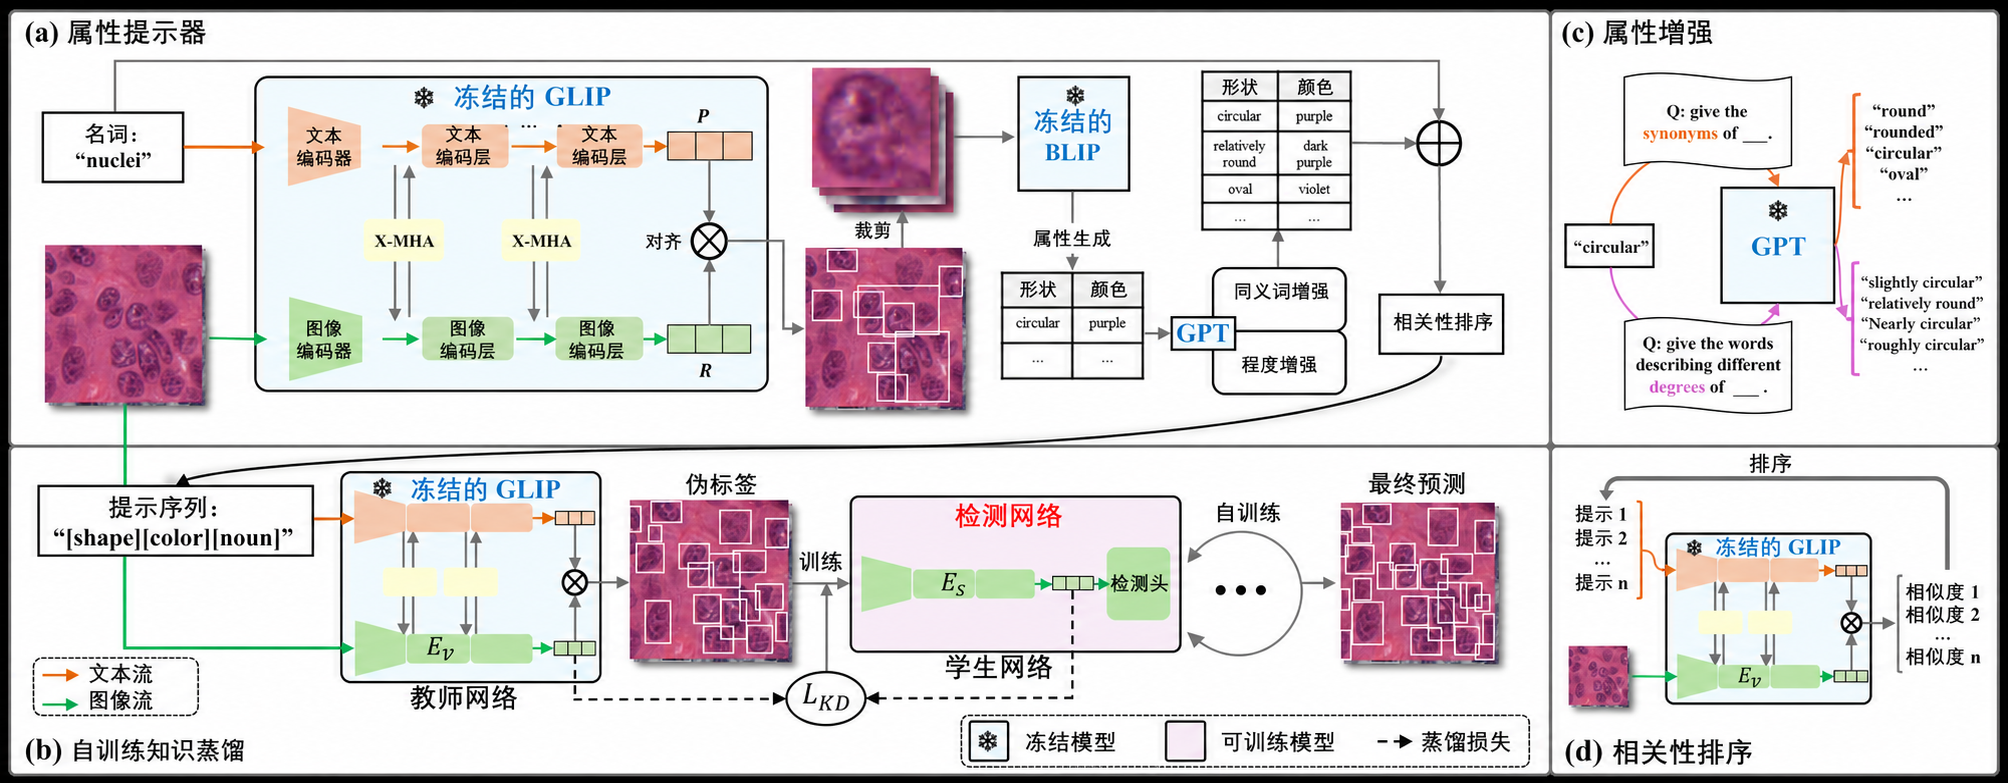
\includegraphics[width=\textwidth]{chapters/PAPERS/nucleiprompter__TMI_final_version/xu1_zh.png}
\caption{AttriPrompter 与知识蒸馏总体框架}
\label{fig:attrip_framework}
\end{figure*}
图~\ref{fig:attrip_framework} 中，(a) 使用 GLIP 和 BLIP 自动生成属性，利用语言模型进行属性增强，并对候选提示进行相关性排序；(b) 基于自训练知识蒸馏进行迭代优化；(c) 属性增强过程；(d) 相关性排序过程。


\subsection{属性生成}

属性生成的目标是从无标注图像中获得能够描述目标外观的词汇，避免依赖病理专家手工设计提示。具体步骤如下。

首先，将 ``nuclei'' 等医学名词作为初始提示输入 GLIP，得到细胞核的粗略候选框。此时的预测不要求具有很高的召回率，其作用是提供可供分析的候选区域。其次，将粗略候选框对应的图像区域裁剪为图像块，并输入冻结的 BLIP。BLIP 是一个兼具图像理解和文本生成能力的视觉语言模型，可以通过视觉问答回答图像块中目标的颜色和形状问题。最后，对 BLIP 生成的词汇进行词频统计和类别筛选，保留最能描述细胞核形状和颜色的属性词。

该流程具有两个优点。一方面，属性直接从目标域图像中提取，能够反映不同染色和成像条件下的细胞核外观；另一方面，属性生成依赖已经完成图文对齐的视觉语言模型，生成的词汇更有可能与 GLIP 的语义空间兼容。与完全人工设计相比，该方法减少了提示选择中的经验偏差，并保留了可解释性：每个最终提示都可以追溯到形状、颜色及其程度属性。

\subsection{属性增强}

属性生成得到的词汇数量和表达方式仍然有限。为扩大语义覆盖范围，AttriPrompter 对属性词执行同义增强和程度增强。

\textbf{同义增强。} 同义词可以在不改变基本语义的情况下提供多种语言表达。本章使用预训练语言模型对属性词进行扩展，例如将描述形状或颜色的常用词扩展为多个可能的自然语言表达。增强提示时使用的约束是：新词应当能够描述 H\&E 染色病理图像中的细胞核，而不是仅仅提供词典意义上的同义词。这样可以避免生成与目标外观无关的词汇。

\textbf{程度增强。} 仅使用 ``round'' 或 ``purple'' 等基本属性，仍然不能区分属性的强弱和程度。程度增强为每个属性添加更细粒度的描述，例如颜色的深浅、形状的圆整程度和弯曲程度。图~\ref{fig:attrip_augmentation} 中，同一框内的词表示基本语义相近的同义表达，不同框中的词表示属性程度不同。通过程度增强，候选集合覆盖了更宽的语义范围，提高了生成有效提示的概率。

\begin{figure}[t]
\centering
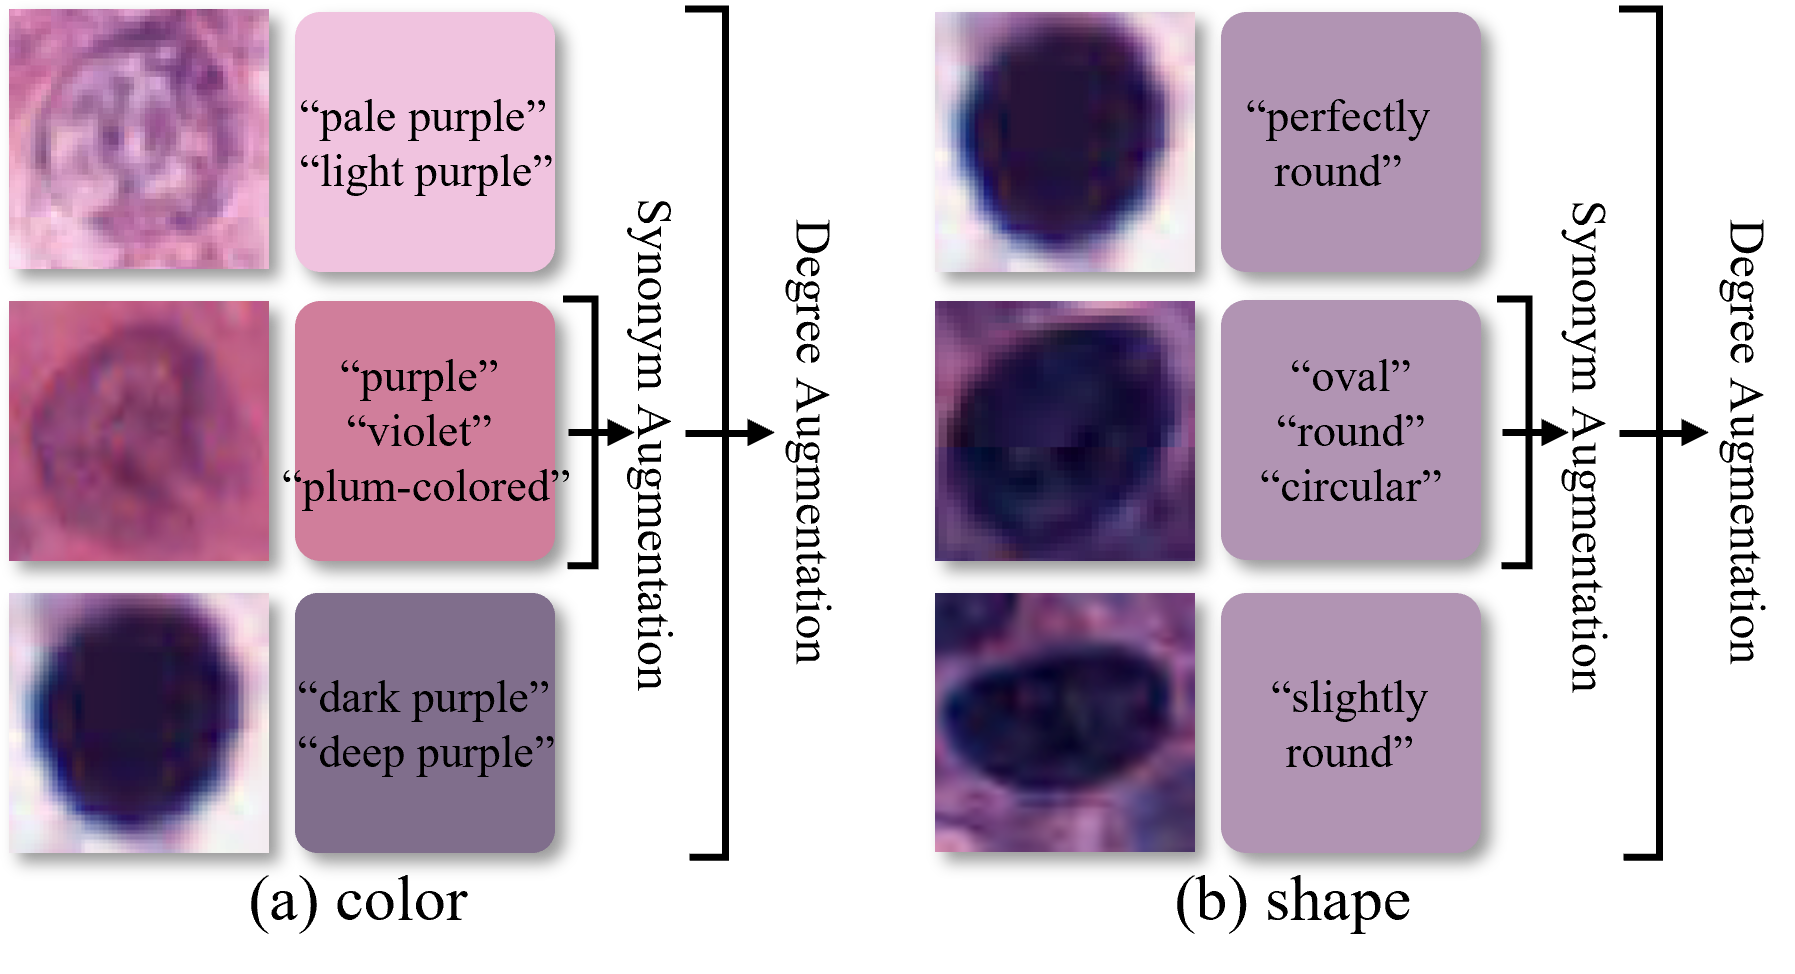
\includegraphics[width=0.95\linewidth]{chapters/PAPERS/nucleiprompter__TMI_final_version/xu3.png}
\caption{属性增强示例}
\label{fig:attrip_augmentation}
\vskip -0.15in
\end{figure}
图~\ref{fig:attrip_augmentation} 中，(a) 对颜色 ``purple'' 的增强；(b) 对形状 ``round'' 的增强。同一框中的词表示同义表达，不同框中的词表示不同程度的属性描述。


\subsection{相关性排序}

将形状属性、颜色属性和医学名词按照模板 ``[shape] [color] [noun].'' 组合，可以形成候选检测提示。但是，程度增强也可能引入与当前图像域相关性较低的词汇。为降低无关提示带来的噪声，AttriPrompter 使用 GLIP 的视觉和文本编码结果计算提示相关性。

设训练图像 $x_i$ 中的候选区域集合为 $\mathcal{B}_i$，候选提示为 $t$。记区域 $b$ 的视觉嵌入为 $R_{i,b}=E_{\mathcal V}(x_i,b)$，提示的文本嵌入为 $P_t=E_{\mathcal T}(t)$，则候选提示在训练集上的平均相关性定义为：
\begin{equation}
\label{eq:attrip_relevance}
s(t)=\frac{1}{\sum_{i=1}^{n}|\mathcal{B}_i|}
\sum_{i=1}^{n}\sum_{b\in\mathcal{B}_i}
\frac{R_{i,b}\cdot P_t}{\|R_{i,b}\|_2\|P_t\|_2}.
\end{equation}

其中，$n$ 为用于提示生成和排序的训练图像数量。原论文为简化记号，将候选区域索引省略；式~\ref{eq:attrip_relevance} 将其显式写出，以说明相关性是对训练图像中的候选区域进行平均，而不是只计算整幅图像的单个相似度。根据 $s(t)$ 对候选提示进行降序排列，选取前 $N$ 个提示输入 GLIP。本章实验中 $N=9$，该值由 MoNuSeg 上的交叉验证确定。

相关性排序并不改变候选提示的文字内容，而是利用目标域图像确定提示的优先级。当相关性高的提示位于序列前部时，GLIP 的跨模态融合更容易先关注与当前图像外观一致的语义描述，从而改善初始预测的稳定性。

\section{知识蒸馏与自训练方法}

\subsection{问题与总体思路}

H\&E 图像中的细胞核通常呈高密度排列，许多相邻实例之间只有很小的间隔。GLIP 虽然具有良好的目标级跨模态表示，但其预训练结构并不是专门为密集同类目标设计的，直接使用 GLIP 预测仍然容易出现漏检、误检和相邻实例重叠。若直接对目标域图像进行普通微调，又可能破坏 GLIP 原有的开放词汇知识。

为此，本章引入自训练知识蒸馏框架。GLIP 作为教师网络，通过 AttriPrompter 生成初始预测；这些预测被视为无人工标注的伪标签。随后，使用检测专用的学生网络学习伪标签，同时通过特征蒸馏损失约束学生特征与 GLIP 图像编码器特征之间的差异。学生网络的结构可以针对密集目标进行选择，实验中主要使用 YOLOX，也验证了 Mask R-CNN 的可替代性。学生网络收敛后重新生成伪标签，并开启下一轮训练，形成迭代自训练过程。

\subsection{教师网络、学生网络与训练目标}

设输入图像为 $x_i$，AttriPrompter 和 GLIP 产生的初始伪标签集合为
\begin{equation}
O_i=\{o_1,\ldots,o_{k_i}\},
\end{equation}
其中 $k_i$ 是第 $i$ 张图像中的伪标签数量。记 GLIP 的图像特征提取器为 $E_{\mathcal V}$，学生网络的特征提取器为 $E_{\mathcal S}$，学生检测头为 $\mathcal H$。知识蒸馏损失采用教师和学生特征之间的 $L_1$ 距离：
\begin{equation}
\label{eq:attrip_kd}
L_{KD}=\left\|E_{\mathcal V}(x_i)-E_{\mathcal S}(x_i)\right\|_1.
\end{equation}

学生网络的整体训练目标为：
\begin{equation}
\label{eq:attrip_student}
L_{\mathcal S}=\frac{1}{n}\sum_{i=1}^{n}
L_{Det}\left(O_i,\mathcal H(E_{\mathcal S}(x_i))\right)
+\alpha L_{KD},
\end{equation}
其中，$L_{Det}$ 表示学生检测网络的检测损失，$\alpha$ 为知识蒸馏损失权重。本章实验将 YOLOX 的特征提取器修改为与 GLIP 图像编码器相同的结构，并使用 GLIP 预训练权重进行初始化，以便进行特征对齐。需要强调的是，GLIP 在这里是教师网络，YOLOX 或 Mask R-CNN 是学生检测网络；SKD 的作用不是重新训练 GLIP，而是将其目标级知识迁移到更适合密集目标检测的网络中。

\subsection{迭代自训练}

第一轮训练结束后，使用已经收敛的学生网络重新预测训练图像，得到更新后的伪标签集合 $O_i^{(r+1)}$。随后以更新后的伪标签启动下一轮学生网络训练：
\begin{equation}
\label{eq:attrip_iterative}
L_{\mathcal S^{(r+1)}}=\frac{1}{n}\sum_{i=1}^{n}
L_{Det}\left(O_i^{(r+1)},
\mathcal H^{(r+1)}(E_{\mathcal S^{(r+1)}}(x_i))\right)
+\alpha L_{KD}.
\end{equation}

从优化角度看，这一过程可以理解为交替更新伪标签和学生网络参数：固定当前模型生成伪标签，再固定伪标签训练下一轮模型。由于后续轮次使用了学生网络对目标形态的建模能力，预测框的位置和数量可以逐步得到修正。实际实验中并非轮次越多越好，因此本章同时报告不同自训练轮次的结果，并根据验证集表现选择最终轮次。

\section{预测反馈驱动的语义闭环与任务扩展方法}

前述实验主要从属性词生成、相关性排序和知识蒸馏三个方面改善零样本细胞核检测。本节进一步研究一个更具一般性的问题：模型在目标域产生的预测结果，能否从单向输出转化为下一轮推理的可用知识。传统零样本检测通常遵循“文本提示输入--视觉语言匹配--检测结果输出”的单向流程，一旦提示确定，目标域图像只能被动接受预训练模型的判别边界。对于病理图像而言，这一范式存在明显局限。自然图像预训练形成的类别语义相对稳定，而细胞核的颜色、形态、尺度和密度会随器官、染色批次及扫描设备变化；固定文本所描述的是跨数据集的概念先验，当前图像中的高置信度实例则包含目标域特有的视觉后验。若能够把后验信息重新写回提示或模型参数，就有可能形成从“语义先验”到“视觉后验”再返回“条件化推理”的闭环。

基于这一认识，本节设计四组相互衔接的研究性实验。第一组冻结模型参数，将高置信度检测框对应的 $256$ 维区域特征聚合为类别原型，并作为模板 token 注入下一轮提示，实现快速、无训练的表示空间适配。第二组进一步允许 GLIP 使用上一轮伪标签更新参数，考察短时原型记忆与慢时参数学习能否形成互补。第三组在共享检测语义的基础上连接轻量级实例分割头，验证框级定位知识能否向像素级边界推理迁移。第四组使用中文视觉语言权重和翻译后的中文医学提示，对英文 GLIP 候选框进行语义重排序，分析语言、预训练语料与医学复合词表达之间的关系。

这四组实验对应三种不同时间尺度的适配机制：模板 token 在单次或少数几次推理内更新，属于快速状态变量；教师--学生训练通过梯度下降改变网络参数，属于慢速结构变量；中文视觉语言重排序不改变 GLIP 定位器，而是替换或补充外部语义先验。通过把三者分开评价，可以判断性能变化究竟来自目标位置被重新发现、类别语义被重新校准，还是网络参数真正吸收了目标域结构。所有实验均保持原始训练集与验证集划分不变，目标域验证标注只用于最终评价，不参与提示构建或参数更新。

\subsection{无训练的框特征模板迭代}

\subsubsection{方法动机与原型记忆}

文本提示提供的是类别层面的抽象描述，例如“深紫色”“近圆形”和“细胞核”；然而，检测器真正需要判断的是某一张目标图像中的局部区域是否与这些描述一致。由于染色风格和成像条件发生变化，同一文本 token 在目标域中的最优视觉对应关系并不固定。高置信度检测框虽然不是人工标注，却是当前模型在目标图像上找到的、与文本语义较一致的实例。其区域特征同时携带颜色、纹理、尺度和局部上下文，因此可以被视为目标域类别分布的经验样本。

对第 $t$ 轮推理中置信度不低于阈值 $\tau$ 的预测框，按类别保留得分最高的 $K=5$ 个实例。根据预测框对应的特征层级和空间位置，从检测头的融合视觉特征中读取 $256$ 维框特征 $\boldsymbol z_i\in\mathbb{R}^{256}$，并以检测置信度 $s_i$ 加权形成类别原型
\begin{equation}
\boldsymbol p_c^{(t)}=
\frac{\sum_{i\in\mathcal I_c}s_i\boldsymbol z_i}
{\sum_{i\in\mathcal I_c}s_i}.
\end{equation}
置信度加权用于抑制边界样本对原型中心的扰动，使原型更接近当前模型认为最典型的类别区域。为减少单张图像偶然误检的影响，进一步使用动量系数 $\beta=0.9$ 更新跨图像原型记忆
\begin{equation}
\boldsymbol m_c^{(t)}
=\beta\boldsymbol m_c^{(t-1)}
 +(1-\beta)\boldsymbol p_c^{(t)}.
\end{equation}
随后将归一化后的原型写入该类别短语末尾的保留 token 位置，并与已经映射到视觉语言对齐空间的文本特征按 $\alpha=0.5$ 混合，再执行下一轮检测。整个过程冻结 GLIP 的全部参数，不进行反向传播。

从统计学习角度看，文本特征可以理解为由大规模预训练语料提供的类别先验，框特征原型则近似表示目标图像条件下的类别后验均值。二者混合相当于在不重新估计全部网络参数的情况下，对类别中心进行经验贝叶斯式修正。从迭代优化角度看，该过程也具有类似期望最大化的结构：当前提示负责产生隐变量形式的实例分配，高置信度实例用于估计新的类别中心，更新后的中心再用于下一轮实例分配。二者并非严格等价，因为检测框不是真实潜变量且不存在显式似然函数，但这一视角能够解释为什么单类别、初始检测较可靠时通常更容易获得收益。

\subsection{GLIP 作为学生网络的闭环自训练}

\subsubsection{双时间尺度适配机制}

无训练模板迭代只改变本轮推理使用的类别表示，优点是速度快、不会破坏预训练参数，缺点是记忆持续时间有限，且无法改变候选框生成器本身。为此，本实验进一步引入教师--学生式参数更新。教师仍为带最优属性提示的 GLIP，并在 CoNSeP 的 108 张训练图像上执行两轮框特征模板推理；以 0.5 为伪标签阈值，共保留 786 个高置信度框，覆盖全部训练图像。学生网络不再使用 YOLOX，而是采用与教师相同的 GLIP 结构并从原始预训练权重初始化，在伪标签上训练 4 个 epoch。测试阶段分别关闭和开启框特征模板，以分离参数更新和原型记忆的贡献。该设置严格使用训练划分生成伪标签，并在独立验证划分上评价，不读取验证标注参与训练。

选择 GLIP 自身作为学生网络具有两点意义。其一，教师和学生共享语言编码、跨模态融合及候选框表示，伪标签从教师到学生的传递不需要跨架构转换，可以减少 YOLOX 等纯视觉学生与视觉语言教师之间的表示失配。其二，学生仍然保留文本条件化能力，训练后不仅学习“哪些位置更像细胞核”，还能够继续接受属性提示和模板 token，从而形成参数空间与提示空间的双重更新。

可将这一过程写为两个不同时间尺度的状态变量。慢变量 $\boldsymbol\theta^{(t)}$ 表示 GLIP 参数，由伪标签集合 $\widetilde{\mathcal D}^{(t)}$ 上的检测损失更新；快变量 $\boldsymbol m_c^{(t)}$ 表示类别原型，在推理阶段根据当前图像即时更新：
\begin{equation}
\boldsymbol\theta^{(t+1)}
=\boldsymbol\theta^{(t)}
-\eta\nabla_{\boldsymbol\theta}
\mathcal L_{\mathrm{det}}
(\boldsymbol\theta^{(t)};\widetilde{\mathcal D}^{(t)}),
\end{equation}
\begin{equation}
\widehat{\mathcal Y}^{(t+1)}
=f_{\boldsymbol\theta^{(t+1)}}(
\boldsymbol x\mid\boldsymbol q,\boldsymbol m^{(t)}).
\end{equation}
参数更新把训练集中反复出现的稳定结构固化到候选框生成和分类边界中；原型记忆则保留对当前图像局部外观的快速适配能力。因此，二者分别回答“训练集上长期稳定的目标结构是什么”和“当前图像中的目标具体长什么样”。

\subsection{带实例分割头的任务扩展}

前两组实验关注“检测到什么”和“检测在哪里”，但细胞核分析还需要精确描述实例边界。检测框只提供低频空间约束，无法区分相邻细胞核之间的接触边界，也不能直接计算面积、圆度和核质比等病理形态量。为验证本章方法并非只能输出检测框，在 GLIP 主干后连接轻量级 tiny mask 头，并在 MoNuSeg 测试划分得到的 224 个图像块上进行实例级评价。该分支从候选框对应的多尺度视觉特征预测实例掩膜，检测与分割共享同一主干和类别语义。

这一扩展的理论依据在于框级视觉语言对齐与像素级形状预测具有层次关系。文本提示首先约束候选区域的类别语义，使模型在大范围图像中找到潜在细胞核；掩膜头随后在候选框限定的局部坐标系中学习前景/背景边界。候选框相当于为像素分类提供空间先验，显著缩小搜索区域；多尺度特征则同时保留低层边缘纹理和高层语义。对于细胞核这类尺度较小、内部纹理相对一致的目标，先定位后分割能够减少组织背景对边界学习的干扰。

\subsection{中文权重与中文医学提示的跨语言验证}

\subsubsection{研究问题与语义分解}

前三组实验都在英文视觉语言预训练权重下进行。本实验进一步检验：将医学提示翻译为中文，并使用中文视觉语言权重进行图文对齐，能否改善病理图像中的目标语义判断。实验采用 Chinese-CLIP 的 ViT-L/14 模型，其图像编码器与中文 RoBERTa 文本编码器在大规模中文图文对上进行对比预训练\cite{yang2022chineseclip}。需要特别说明的是，该权重并不是 GLIP 的中文检测版本，因此本文不直接用它替换 GLIP 检测器，而采用“GLIP 定位候选框 + Chinese-CLIP 中文语义重排序”的解耦结构。这样既保持 GLIP 已有的区域定位能力，又真实使用中文图像编码器、中文文本编码器和中文提示进行语义比较。

本实验的动机不应被简化为“中文表意而英文表音，因此中文天然优于英文”。英语医学术语同样具有稳定的形态和词源结构，模型性能主要受分词方式、预训练语料、视觉域差异和文本描述粒度共同影响。更严谨的假设是：部分中文病理复合词能够在较短序列中显式组合结构、形态和染色属性，例如“血管内皮细胞核”“细长梭形”“深染”“高度异型”等；当中文文本编码器在足够规模的中文图文语料上训练后，这些属性组合可能形成不同于英文提示的语义邻域。实验要验证的不是中文语言本身的普遍优越性，而是中文权重和中文医学提示作为另一种语义先验，能否补充英文 GLIP 在病理小目标上的类别判断。

对于类别 $c$，将英文提示翻译并扩展为 $M$ 条中文医学描述 $q_{c,m}^{\mathrm{zh}}$。使用中文文本编码器 $f_T^{\mathrm{zh}}$ 得到类别原型
\begin{equation}
\boldsymbol p_c^{\mathrm{zh}}
=\operatorname{Norm}\left(
\frac{1}{M}\sum_{m=1}^{M}
f_T^{\mathrm{zh}}(q_{c,m}^{\mathrm{zh}})
\right).
\end{equation}
多描述平均的目的不是简单增加文本长度，而是降低单一翻译措辞带来的方差，使类别中心同时包含名称、染色、形状和组织位置等互补属性。对 GLIP 产生的第 $i$ 个候选框，在其外侧保留 $10\%$ 上下文并裁剪图像，使用 Chinese-CLIP 图像编码器得到区域特征 $\boldsymbol v_i^{\mathrm{zh}}$，语义相似度为
\begin{equation}
r_{i,c}^{\mathrm{zh}}
=\frac{
\exp(\boldsymbol v_i^{\mathrm{zh}\top}
\boldsymbol p_c^{\mathrm{zh}}/T)}
{\sum_{c'}\exp(
\boldsymbol v_i^{\mathrm{zh}\top}
\boldsymbol p_{c'}^{\mathrm{zh}}/T)}.
\end{equation}
最后，将 GLIP 定位置信度 $s_i^{\mathrm{loc}}$ 与中文语义置信度按几何平均融合：
\begin{equation}
s_{i,c}
=(s_i^{\mathrm{loc}})^{1-\lambda}
(r_{i,c}^{\mathrm{zh}})^{\lambda}.
\end{equation}
该形式将定位与识别明确分离。当 $\lambda$ 较小时，系统主要保留 GLIP 的候选框排序，中文分支只提供弱语义校准；当 $\lambda$ 较大并加入背景类别时，中文分支可以直接否决候选框，形成强语义门控。

\section{实验设置}

\subsection{数据集与数据划分}

\textbf{MoNuSeg。} MoNuSeg 包含 30 张 $1000\times1000$ 像素的细胞核图像，每张图像平均包含约 658 个细胞核。按照数据集原始划分，使用 16 张图像训练，14 张图像测试；训练过程中每个 epoch 随机选择 4 张图像用于验证。每张大图提取 16 个具有重叠区域的 $256\times256$ 图像块，并随机裁剪为 $224\times224$ 作为模型输入。训练图像仅用于自动提示生成和伪标签自训练，测试图像及其真实标注只用于最终评估。

\textbf{CoNSeP。} CoNSeP 是面向结直肠细胞核分割和表型分析的数据集，包含 41 张 $1000\times1000$ 像素的 H\&E 染色图像，这些图像来自 16 张结直肠腺癌全视野切片。除非另有说明，本章沿用与 MoNuSeg 相同的预处理方式。按照数据集默认划分，使用 26 张图像训练、1 张图像验证、14 张图像测试。

\subsection{评价指标}

本章遵循 COCO 评价协议，采用平均精度 mAP、IoU 阈值为 0.50 的 AP50、IoU 阈值为 0.75 的 AP75，以及平均召回率 AR 作为主要检测指标。mAP 综合多个 IoU 阈值下的精度，反映预测框定位精度与置信度排序的整体质量；AP50 更关注较宽松的目标匹配，AP75 对定位误差更敏感；AR 则用于衡量模型发现目标的能力。对于伪标签分析，额外使用每个伪标签与真实实例中最大 IoU 的平均值 $\mathrm{mIoU}_{\mathrm{nearest}}$，以区分“定位较准但数量不足”和“定位本身不准”两类情况。

\subsection{实现细节}

除非另有说明，实验使用 4 张具有 24 GB 显存的 NVIDIA RTX 3090 GPU。AttriPrompter 的属性生成使用在 ViT-B 和 CapFilt-L 上微调的 BLIP VQA 权重，视觉问答问题分别为 ``what is the color of the nuclei'' 和 ``what is the shape of the nuclei''。属性增强使用 ChatGPT 3.5，提示内容分别要求生成“能够描述 H\&E 染色病理图像中细胞核的同义词”和“描述某一属性不同程度的词语”。相关性排序选取 $N=9$ 个提示。主干视觉语言模型使用 GLIP-L。

在 SKD 中，将 YOLOX 的特征提取器替换为与 GLIP 图像编码器一致的结构，并使用 GLIP 预训练参数初始化；学生网络的其他训练设置采用 YOLOX 默认配置。知识蒸馏权重 $\alpha=1$，该值通过 MoNuSeg 上的四折交叉验证确定。若未特别说明，每张图像最多保留 20 个伪标签。不同的自训练轮次均使用相同的评价协议，避免把轮次变化和评价方法变化混在一起。

为便于复现，本章同时核对了当前 GLIP 工程中的任务配置。检测器采用 GeneralizedVLRCNN 总体结构，视觉分支由 Swin Transformer、FPN 和 256 通道 DyHead 组成，DyHead 包含 8 个动态卷积层并在各特征层保留前 9 个正样本候选；语言分支采用 BERT-base-uncased，视觉与文本特征通过早期 MHA-B 跨模态融合。输入图像的训练与测试短边统一为 800 像素，使用 AdamW 优化器；论文主实验沿用 GLIP-L 预训练权重，补充的实例分割实验则开启轻量掩膜分支，ROI 特征分辨率为 $14\times14$，掩膜输出分辨率为 $28\times28$。命令行中设置的学习率、批大小、训练轮数和检查点周期优先于配置文件默认值，因而每组对比实验均以实际运行参数为准，而不直接沿用配置文件中的占位训练上限。

\subsection{补充实验方案与控制变量}
四组补充实验分别检验无训练模板 token、GLIP 教师--学生闭环、实例分割头和中文医学提示。各实验沿用既定训练集、验证集和测试集划分；验证集标注只用于评价，不参与模板构建、伪标签生成或参数更新。涉及多轮反馈时，固定首轮提示、置信度阈值和最大候选数量，并同时报告精度与召回率，避免只根据单一指标选择有利结果。

\subsection{跨域实验协议}

医学图像可能来自不同医疗中心、扫描设备或染色流程，域偏移会改变细胞核的颜色、纹理和形状分布。因此，本节开展两组跨域实验。第一组实验检验 AttriPrompter 本身的跨域能力：使用一个数据集生成提示，再在另一个数据集上进行 SKD 和测试。第二组实验检验完整系统的 domain shift 性能：在源域训练整个系统，在不同目标域测试。实验流程如图~\ref{fig:attrip_cross_domain} 所示。

\begin{figure}[t]
\centering
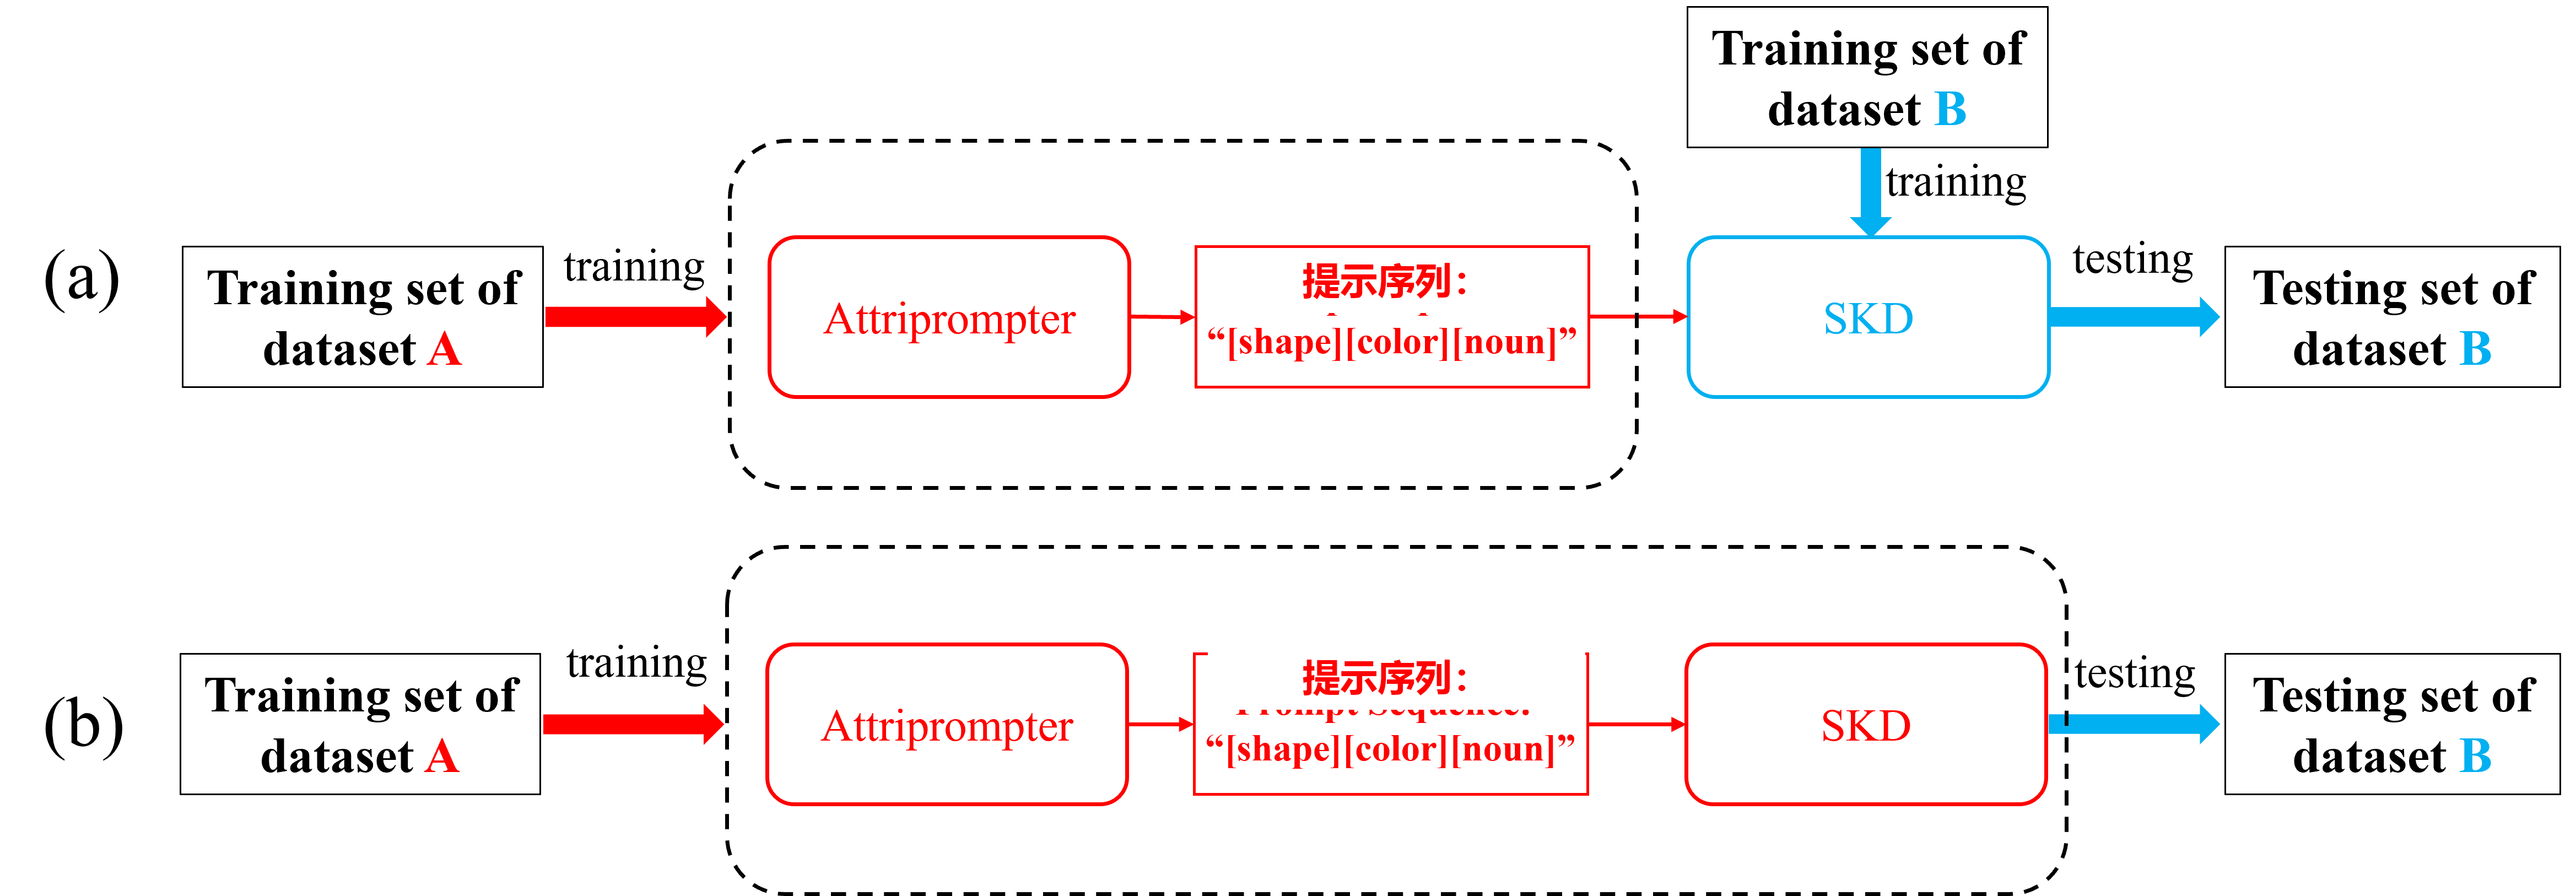
\includegraphics[width=\linewidth]{chapters/PAPERS/nucleiprompter__TMI_final_version/xu5_zh.png}
\caption{跨域实验设置}
\label{fig:attrip_cross_domain}
\end{figure}
图~\ref{fig:attrip_cross_domain} 中，(a) 验证 AttriPrompter 的跨域能力；(b) 验证完整系统的 domain shift 性能。数据集 A 和数据集 B 分别表示源域和目标域。

\section{实验结果与分析}

\subsection{提示语义与顺序的先验分析}
\subsubsection{语义描述粒度的影响}

在 MoNuSeg 测试集上，分别使用仅包含类别名、加入基本形状和颜色、以及进一步加入程度描述的文本提示。结果如表~\ref{tab:attrip_PAdegree} 所示。

\begin{table}[t]
\caption{文本提示粒度对检测性能的影响}
\label{tab:attrip_PAdegree}
\begin{center}
\begin{small}
\resizebox{0.75\columnwidth}{!}{
\begin{tabular}{cc}
\toprule[1.5pt]
\textbf{文本提示} & \textbf{mAP} \\ \midrule[1.2pt]
``Nuclei.'' & 0.034 \\
``Round purple nuclei.'' & 0.046 \\
``Relatively round dark purple nuclei.'' & 0.115 \\ \bottomrule[1.5pt]
\end{tabular}
}
\end{small}
\end{center}
\vskip -0.1in
\end{table}
表~\ref{tab:attrip_PAdegree} 中，提示从上到下逐步增加语义描述的细节。


仅使用 ``Nuclei.'' 时，GLIP 的预测较为粗糙，并且容易在背景区域产生响应。加入 ``round'' 和 ``purple'' 后，检测性能有所提升，说明形状和颜色属性可以帮助模型缩小目标语义范围。进一步加入 ``relatively'' 和 ``dark'' 等程度描述后，mAP 从 0.046 提升到 0.115，表明描述属性的程度和细粒度同样重要。这里的程度描述不只是增加文本长度，而是为属性提供了方向和强度，例如颜色的深浅、形状的圆整程度等，使候选描述能够覆盖不同外观的细胞核。

\subsubsection{提示序列顺序的影响}

GLIP 通常将多个对象词或短语组织在同一个文本序列中。实验发现，当多个候选提示同时输入时，提示在序列中的位置会影响模型输出。图~\ref{fig:attrip_parelevance} 展示了按照图文相关性排序的提示序列及其预测效果。相关性较高的提示放在前部时，GLIP 的预测精度更高。

\begin{figure}[t]
\centering
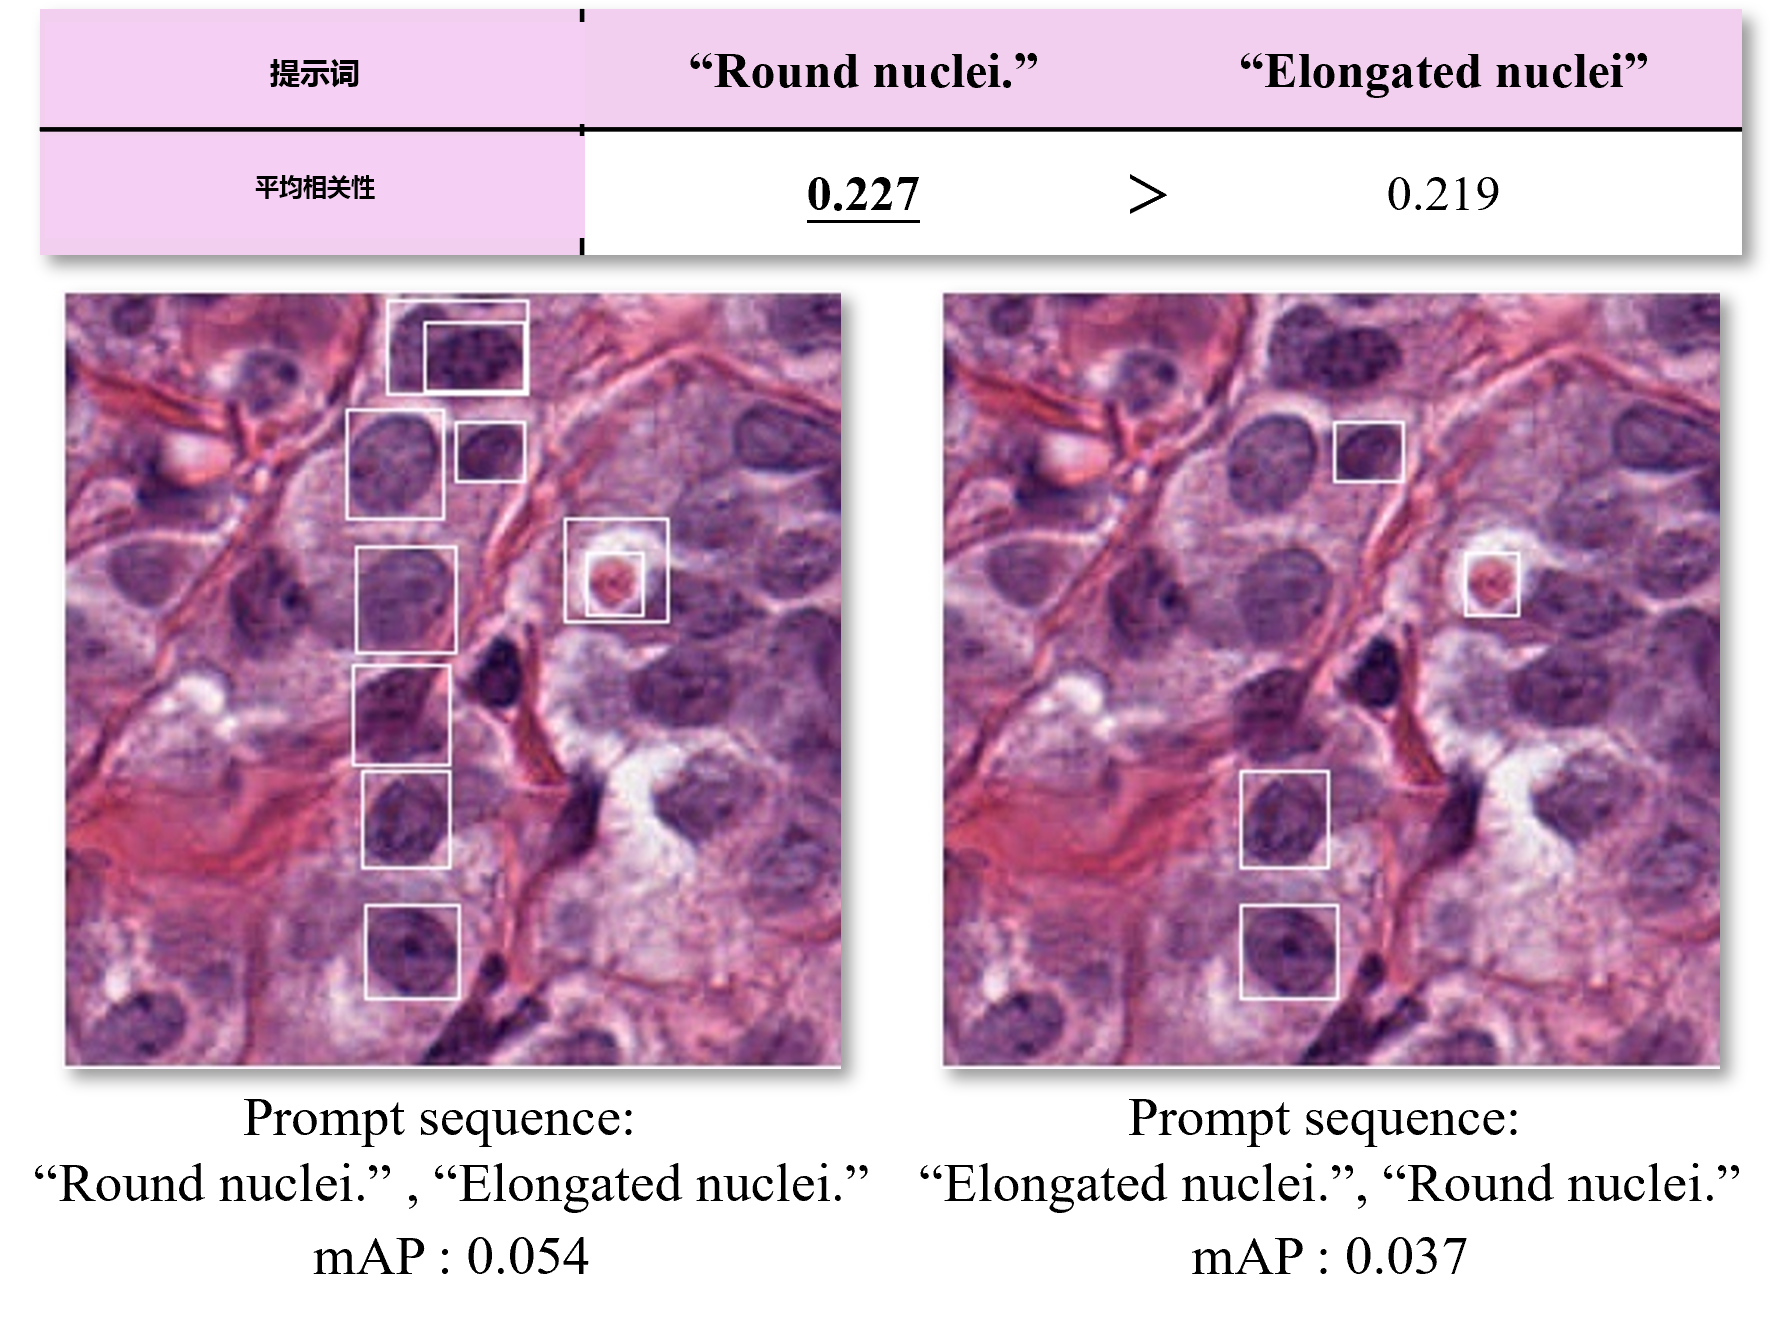
\includegraphics[width=0.95\linewidth]{chapters/PAPERS/nucleiprompter__TMI_final_version/xu2_zh.png}
\caption{提示排序对检测性能的影响}
\label{fig:attrip_parelevance}
\end{figure}
图~\ref{fig:attrip_parelevance} 中，mAP 在 MoNuSeg 测试集上统计。


这一现象说明提示序列并不是候选短语的简单集合。由于跨模态融合过程会受到序列上下文的影响，越符合当前图像域的提示越适合被放在前面。由此，本章将提示构造拆分为属性生成、属性增强和相关性排序三个步骤，以降低人工设计提示的主观性，并使提示序列能够随数据域变化而自动调整。

本节不按方法名称简单罗列结果，而按照误差来源组织分析。首先比较整体检测性能，确定本章方法相对于不同监督强度基线的收益；随后分别考察提示语义、属性组合、伪标签来源、蒸馏损失和学生结构，最后将结论放到跨域场景中检验。这样的组织方式可以区分三类因素：提示是否提供了正确的目标语义，伪标签是否提供了足够可靠的定位监督，以及学生网络是否能够把教师先验转化为稳定的检测能力。

\subsection{与现有方法的比较}

表~\ref{tab:attrip_comparison} 汇总了本章方法与全监督、弱监督以及无监督方法的比较结果。带有 ``*'' 的方法基于医学图像，带有 ``**'' 的方法专门针对 H\&E 图像，其余方法原本面向自然图像，经过适配后用于细胞核检测。弱监督方法使用点标注作为监督信号；本章按照细胞核实例掩膜的中心生成点标注，以保持点监督定义的一致性。

\begin{table}[t]
\caption{MoNuSeg 与 CoNSeP 检测结果}
\label{tab:attrip_comparison}
\begin{center}
\resizebox{\columnwidth}{!}{
\begin{tabular}{ccccccccc}
\toprule[1.5pt]
\multirow{2}{*}{\textbf{方法}} & \multicolumn{4}{c}{\textbf{MoNuSeg}} & \multicolumn{4}{c}{\textbf{CoNSeP}} \\ \cmidrule(r){2-5} \cmidrule(r){6-9}
 & \textbf{mAP} & \textbf{AP50} & \textbf{AP75} & \textbf{AR} & \textbf{mAP} & \textbf{AP50} & \textbf{AP75} & \textbf{AR} \\ \midrule[1.2pt]
\multicolumn{9}{c}{\textbf{全监督基线}} \\
\textbf{YOLOX} & 0.447 & 0.832 & 0.437 & 0.528 & 0.388 & 0.726 & 0.384 & 0.495 \\ \hline
\multicolumn{9}{c}{\textbf{弱监督方法}} \\
\textbf{WSPointA(2019)**\cite{qu2019weakly}} & 0.341 & 0.683 & 0.272 & 0.423 & 0.301 & 0.593 & 0.277 & 0.362 \\
\textbf{WSPPointA(2020)**\cite{qu2020weakly}} & 0.367 & 0.763 & 0.302 & 0.453 & 0.308 & 0.607 & 0.281 & 0.373 \\
\textbf{WSMixedA(2020)**\cite{qu2020nuclei}} & 0.374 & 0.771 & 0.374 & 0.488 & 0.330 & 0.653 & 0.307 & 0.412 \\
\textbf{WNSeg(2022)**\cite{liu2022weakly}} & 0.404 & 0.797 & 0.416 & 0.505 & 0.364 & 0.675 & 0.329 & 0.434 \\ \hline
\multicolumn{9}{c}{\textbf{无监督方法：非视觉语言预训练模型}} \\
\textbf{SSNS(2020)**\cite{sahasrabudhe2020self}} & 0.354 & 0.739 & 0.288 & 0.441 & 0.243 & 0.458 & 0.215 & 0.294 \\
\textbf{PDAM(2020)*\cite{liu2020pdam}} & 0.275 & 0.588 & 0.228 & 0.380 & 0.166 & 0.364 & 0.132 & 0.298 \\
\textbf{DARCNN(2021)*\cite{hsu2021darcnn}} & 0.262 & 0.476 & 0.267 & 0.356 & 0.173 & 0.388 & 0.129 & 0.310 \\
\textbf{Freesolo(2022)\cite{wang2022freesolo}} & 0.292 & 0.607 & 0.248 & 0.393 & 0.222 & 0.393 & 0.246 & 0.370 \\
\textbf{SOP(2022)*\cite{le2022unsupervised}} & 0.235 & 0.609 & 0.096 & 0.351 & 0.171 & 0.387 & 0.127 & 0.304 \\
\textbf{PSM(2022)**\cite{chen2022unsupervised}} & 0.227 & 0.447 & 0.218 & 0.375 & 0.142 & 0.323 & 0.102 & 0.286 \\
\textbf{CutLER(2023)\cite{wang2023cut}} & 0.115 & 0.213 & 0.117 & 0.184 & 0.089 & 0.181 & 0.049 & 0.155 \\ \hline
\multicolumn{9}{c}{\textbf{无监督方法：视觉语言预训练模型}} \\
\textbf{VL-PLM(2022)\cite{zhao2022exploiting}} & 0.333 & 0.582 & 0.342 & 0.501 & 0.159 & 0.357 & 0.120 & 0.291 \\
\textbf{VLDet(2023)\cite{lin2022learning}} & 0.173 & 0.407 & 0.112 & 0.263 & 0.110 & 0.296 & 0.053 & 0.245 \\
\textbf{MIU-VL(2023)*\cite{qin2022medical}} & 0.070 & 0.118 & 0.076 & 0.126 & 0.066 & 0.133 & 0.045 & 0.121 \\
\textbf{VLPM-NuD(2023)**\cite{wu2023zeroshot}} & 0.416 & 0.808 & 0.382 & 0.502 & 0.359 & 0.668 & 0.363 & 0.480 \\
\textbf{本章方法**} & \textbf{0.425} & \textbf{0.819} & \textbf{0.401} & \textbf{0.511} & \textbf{0.367} & \textbf{0.669} & \textbf{0.376} & \textbf{0.488} \\ \bottomrule[1.5pt]
\end{tabular}
}
\end{center}
\end{table}
表~\ref{tab:attrip_comparison} 中，带 ``*'' 的方法基于医学图像，带 ``**'' 的方法专门针对 H\&E 图像。无监督方法中的最优结果以粗体表示。


本章方法在 MoNuSeg 与 CoNSeP 上均取得了无监督方法中的最佳综合结果，并在 mAP、AP50 与 AP75 上整体接近全监督 YOLOX。这说明：在不使用实例标注的前提下，借助视觉语言模型的开放词汇表征与伪标签自训练，仍可以获得较为可靠的“目标级”监督信号。

从误差形态看，非视觉语言的无监督方法（如 SSNS、PDAM、DARCNN、SOP、PSM 等）往往依赖尺寸先验、阈值过滤或特定的域适配假设来生成候选框/伪标注。在细胞核这种“密集、同类、形态差异细微”的场景中，这类规则或弱先验很难同时兼顾两点：一方面要抑制相邻细胞核之间的粘连与重复检测（避免假阳性、提高 AP75），另一方面又要尽可能找全小而弱的细胞核（避免漏检、提高 AR）。因此，这些方法常呈现“定位还可以但数量不足”或“数量尚可但框偏移明显”的权衡。

基于视觉语言预训练的 VL-PLM 与 VLDet 具备开放词汇能力，但其提示设计通常来自自然图像语境，且缺少针对 H\&E 染色下颜色/形态属性的细粒度刻画；再加上它们的检测设定更偏向于中低密度目标，使得在细胞核密集分布时更容易出现置信度排序紊乱、相邻目标混淆等问题，导致 mAP 与 AR 受限。MIU-VL 同样以 GLIP 为基础，但其自动提示更偏向位置或布局属性，适合稀疏目标检测；当细胞核呈现高密度、外观相似且边界模糊时，这类提示可能无法提供足够区分性的语义约束，甚至会引入与“核外观”无关的干扰，从而影响跨模态对齐效果。

AttriPrompter 的收益主要来自三点：其一，自动属性生成让提示能够显式覆盖目标域外观（如颜色深浅、形状趋向等），从语义侧约束 GLIP 的关注区域；其二，同义与程度增强扩大了细粒度语义覆盖，使模型能够在不同染色强度、不同形态变体下保持鲁棒匹配；其三，相关性排序用于抑制低相关或噪声提示，减少文本侧噪声对跨模态融合的负面影响。在此基础上结合 SKD，学生检测器能够吸收 GLIP 的目标级先验，并在多轮伪标签更新中逐步校正框的位置与数量，从而更适配密集细胞核结构。图~\ref{fig:attrip_comparison} 给出了不同方法的检测可视化结果，用于直观对比漏检、重复检测以及定位偏移等典型误差。

\begin{figure*}[t]
\centering
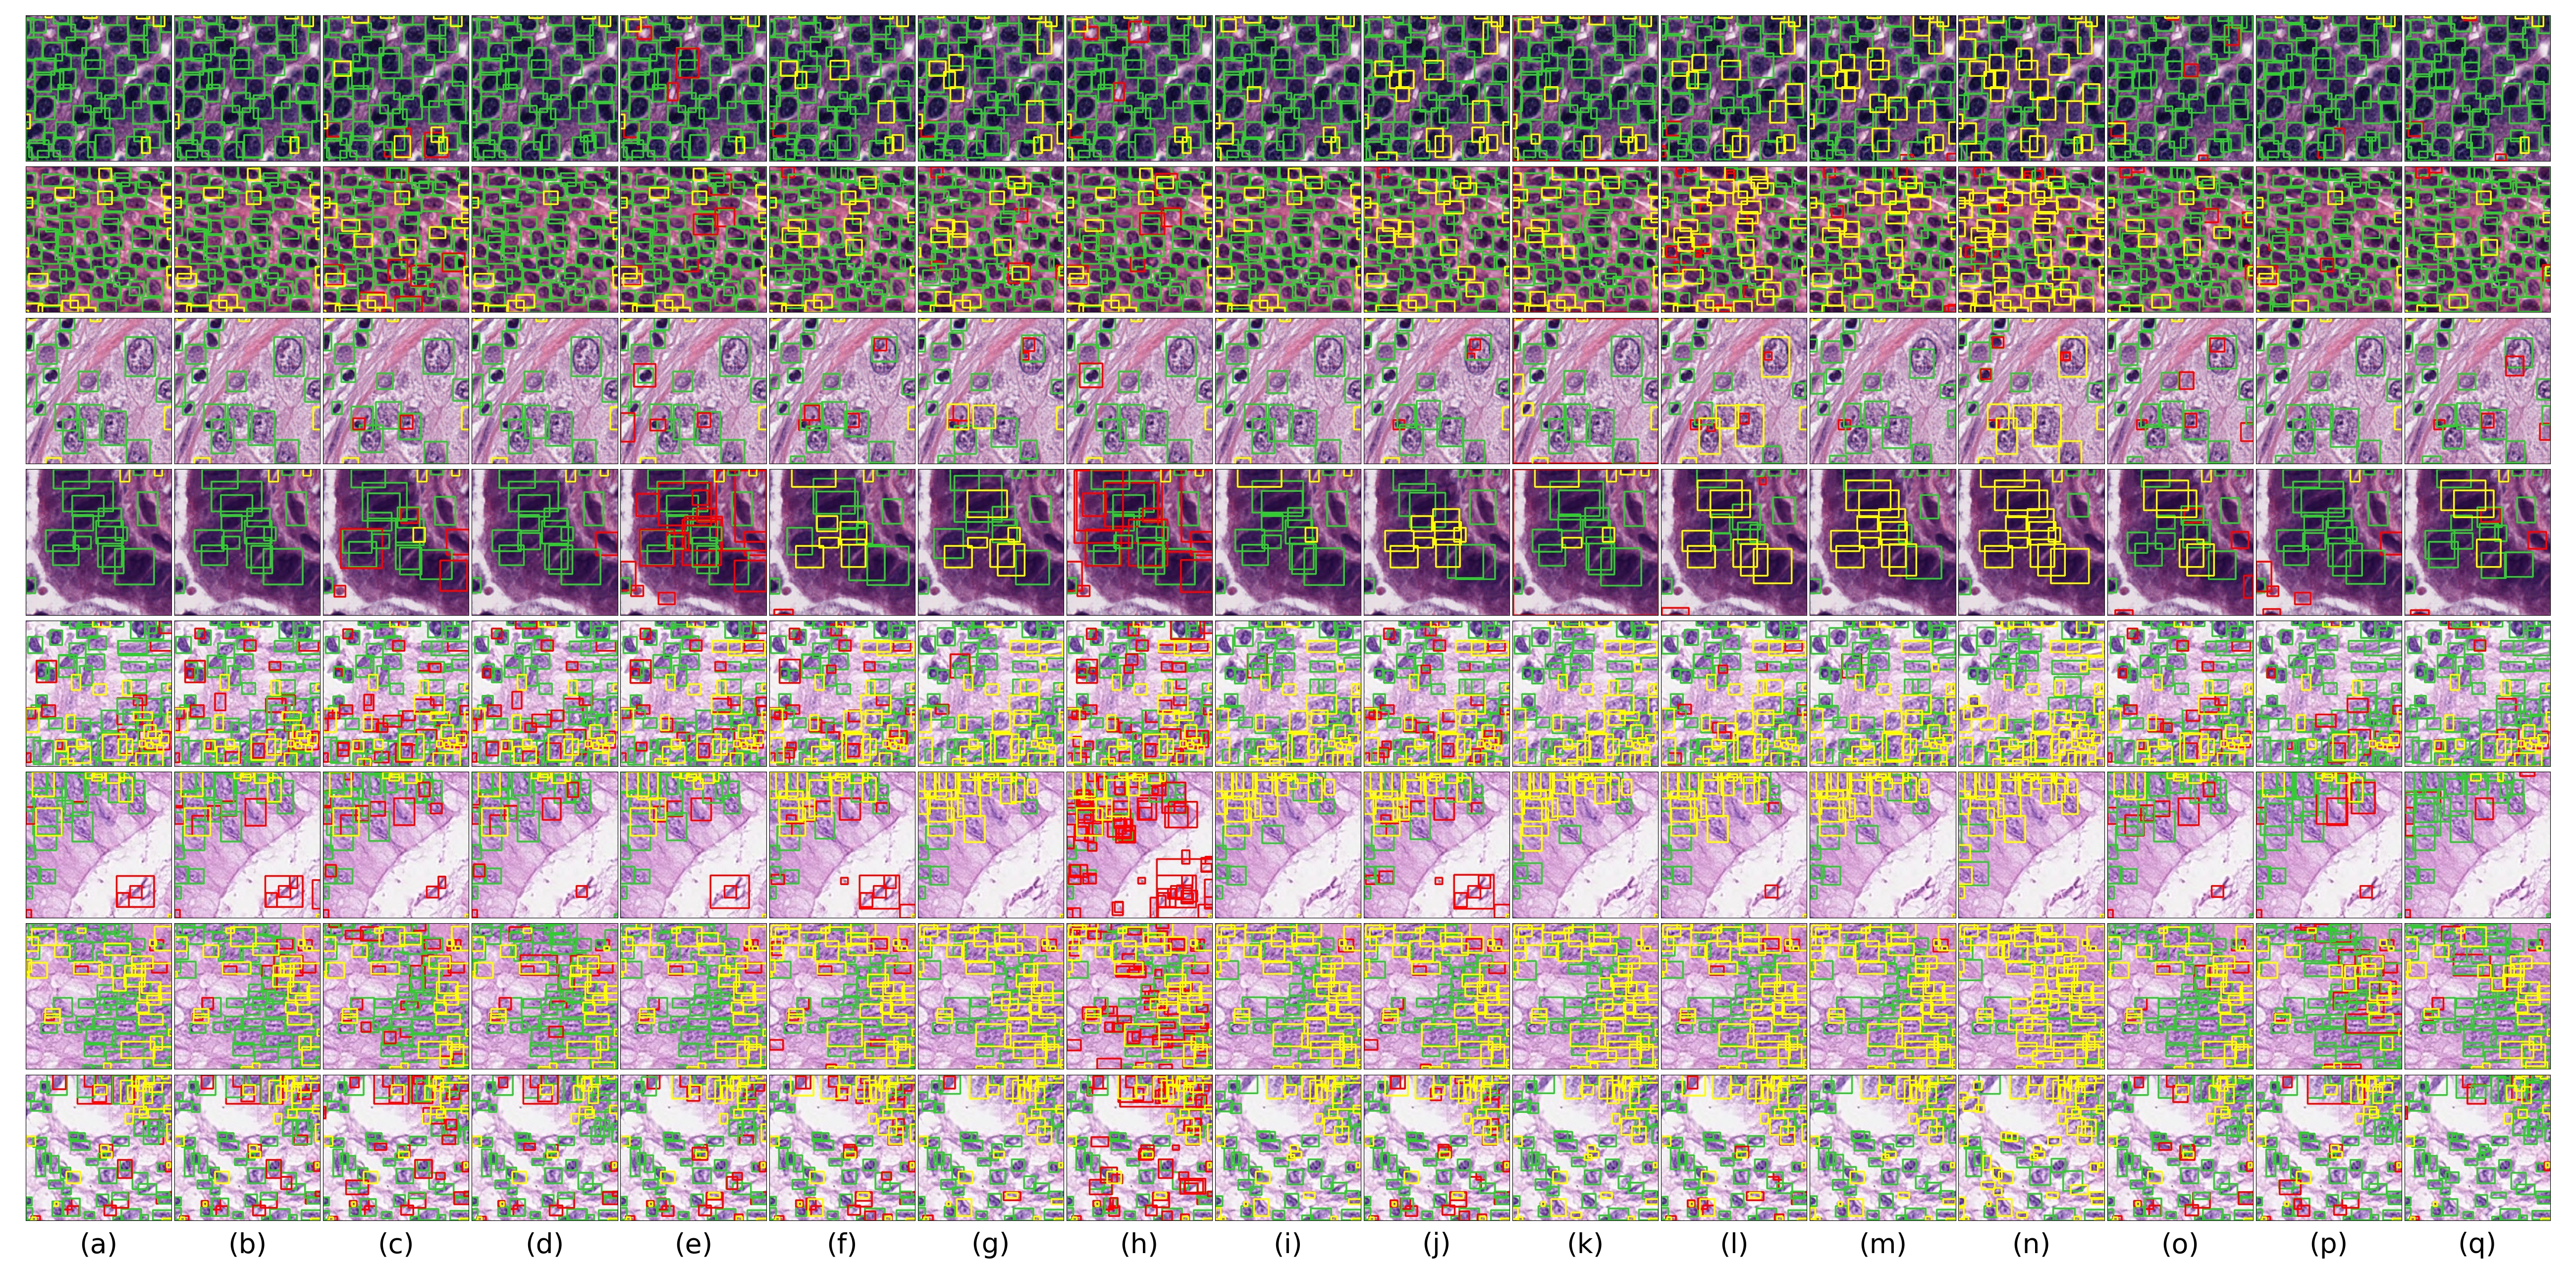
\includegraphics[width=\linewidth]{chapters/PAPERS/nucleiprompter__TMI_final_version/xu4.png}
\caption{跨数据集检测结果可视化}
\label{fig:attrip_comparison}
\end{figure*}
图~\ref{fig:attrip_comparison} 中，前四行为 MoNuSeg，后四行为 CoNSeP。绿色、红色和黄色框分别表示真阳性、假阳性和假阴性。


\subsection{自动提示与人工提示}

为直接评估提示质量，本节不引入 SKD，而是将不同提示序列直接输入 GLIP，并在相同设置下进行零样本检测。人工提示由三位病理专家分别设计，结果取平均值；其描述通常包含染色质形态、核仁以及深蓝或紫色等颜色信息。自动提示则分别使用医学名词、形状属性、颜色属性以及形状和颜色的组合。表~\ref{tab:attrip_prompt} 中的 ``Aug.'' 表示经过语言模型增强。

\begin{table}[t]
\caption{自动提示与人工提示对比}
\label{tab:attrip_prompt}
\begin{center}
\resizebox{0.9\columnwidth}{!}{
\renewcommand{\arraystretch}{1.1}
\begin{tabular}{ccccccc}
\toprule[1.5pt]
\multicolumn{3}{c}{\multirow{2}{*}{\textbf{提示设计}}} & \multicolumn{4}{c}{\textbf{MoNuSeg}} \\ \cline{4-7}
\multicolumn{3}{c}{} & \textbf{mAP} & \textbf{AP50} & \textbf{AP75} & \textbf{AR} \\ \midrule[1.2pt]
\multicolumn{3}{c}{\textbf{人工设计}} & 0.151 & 0.259 & 0.166 & 0.210 \\ \hline
\multirow{10}{*}{\textbf{自动生成}} & \multicolumn{2}{c}{\textbf{MIU-VL(2023)\cite{qin2022medical}}} & 0.070 & 0.118 & 0.076 & 0.126 \\ \cline{2-7}
 & \textbf{属性} & \textbf{名词} & & & & \\ \cline{2-7}
 & \multirow{2}{*}{\textbf{无}} & \textbf{``Nuclei.''} & 0.034 & 0.057 & 0.038 & 0.058 \\
 & & \textbf{Aug. [noun.]} & 0.029 & 0.054 & 0.029 & 0.059 \\ \cline{2-7}
 & \textbf{[shape]} & \textbf{``Nuclei.''} & 0.097 & 0.181 & 0.097 & 0.155 \\
 & \textbf{Aug. [shape]} & \textbf{``Nuclei.''} & 0.124 & 0.255 & 0.124 & 0.191 \\ \cline{2-7}
 & \textbf{[color]} & \textbf{``Nuclei.''} & 0.009 & 0.016 & 0.010 & 0.024 \\
 & \textbf{Aug. [color]} & \textbf{``Nuclei.''} & 0.064 & 0.115 & 0.066 & 0.112 \\ \cline{2-7}
 & \textbf{[shape][color]} & \textbf{``Nuclei.''} & 0.155 & 0.285 & 0.152 & \textbf{0.239} \\
 & \textbf{Aug. [shape][color]} & \textbf{``Nuclei.''} & \textbf{0.179} & \textbf{0.310} & \textbf{0.193} & 0.220 \\ \bottomrule[1.5pt]
\end{tabular}
}
\end{center}
\end{table}
表~\ref{tab:attrip_prompt} 中，该实验不使用 SKD，用于直接评估提示设计质量。最优结果以粗体表示。


结果显示，人工提示能够取得一定性能，但依赖设计者经验，难以保证不同数据域之间的一致性。只使用类别名时性能最低；加入形状或颜色属性后性能总体提升；同时使用形状和颜色时效果最好。值得注意的是，名词同义扩展并未带来收益，可能原因是 ``cyteblast'' 和 ``karyon'' 等生僻词没有充分出现在 GLIP 的预训练语料中。相比之下，常见自然语言属性词更容易与预训练视觉语义形成对应关系。MIU-VL 的表现较低，也说明适合稀疏医学目标的位置类属性不一定适合密集细胞核检测。

\subsection{AttriPrompter 组件消融}

表~\ref{tab:attrip_promptcom} 分别去除同义增强、程度增强和相关性排序，分析三个组件的独立作用及组合效果。所有设置均不使用 SKD，以排除学生网络和自训练过程的影响。

\begin{table}[t]
\caption{AttriPrompter 组件消融}
\label{tab:attrip_promptcom}
\begin{center}
\resizebox{0.9\columnwidth}{!}{
\begin{tabular}{ccccccc}
\toprule[1.5pt]
\textbf{同义增强} & \textbf{程度增强} & \textbf{相关性排序} & \textbf{mAP} & \textbf{AP50} & \textbf{AP75} & \textbf{AR} \\ \midrule[1.2pt]
 & & & 0.150 & 0.275 & 0.150 & 0.228 \\
\checkmark & & & 0.160 & 0.285 & 0.173 & 0.201 \\
 & \checkmark & & 0.176 & 0.304 & 0.187 & 0.213 \\
 & & \checkmark & 0.155 & 0.290 & 0.152 & \textbf{0.239} \\
\checkmark & & \checkmark & 0.174 & 0.301 & 0.188 & 0.210 \\
 & \checkmark & \checkmark & 0.178 & \textbf{0.314} & 0.187 & 0.217 \\
\checkmark & \checkmark & & 0.177 & 0.309 & \textbf{0.193} & 0.220 \\
\checkmark & \checkmark & \checkmark & \textbf{0.179} & 0.310 & \textbf{0.193} & 0.220 \\ \bottomrule[1.5pt]
\end{tabular}
}
\end{center}
\vskip -0.15in
\end{table}
表~\ref{tab:attrip_promptcom} 中，该实验不使用 SKD。最优结果以粗体表示。


三个组件组合使用时 mAP 达到 0.179，是表中最高值。程度增强和相关性排序的组合在 AP50 上达到最高值，说明细粒度属性和提示顺序分别改善了候选语义和序列上下文。仅使用同义增强的设置与第二章中较早的自动提示方案相近，性能提升相对有限。总体而言，程度增强是本章相对于基础自动属性提示的重要扩展，而相关性排序则进一步利用了 GLIP 对提示顺序的敏感性。

\subsection{不同伪标签生成方式的自训练}

为了区分“伪标签质量”和“学生网络自训练能力”的作用，本节比较 Superpixels、MIU-VL 和 AttriPrompter 三种伪标签来源。除伪标签生成方法外，三个设置均使用相同的 YOLOX 自训练框架。表~\ref{tab:attrip_selftraining} 中，Round 0 表示直接将初始伪标签与真实标注比较；Round 1 表示学生网络完成第一轮收敛后的结果；后续轮次使用前一轮学生网络生成新的伪标签。AttriPrompter 列的结果不使用知识蒸馏，以便单独考察伪标签和自训练过程。

\begin{table}[t]
\caption{不同伪标签的自训练结果}
\label{tab:attrip_selftraining}
\begin{center}
\resizebox{\columnwidth}{!}{
\begin{tabular}{ccccccccccccc}
\toprule[1.5pt]
\multirow{2}{*}{\textbf{轮次}} & \multicolumn{4}{c}{\textbf{Superpixels}} & \multicolumn{4}{c}{\textbf{MIU-VL}} & \multicolumn{4}{c}{\textbf{AttriPrompter}} \\ \cmidrule(r){2-5} \cmidrule(r){6-9} \cmidrule(r){10-13}
 & \textbf{mAP} & \textbf{AP50} & \textbf{AP75} & \textbf{AR} & \textbf{mAP} & \textbf{AP50} & \textbf{AP75} & \textbf{AR} & \textbf{mAP} & \textbf{AP50} & \textbf{AP75} & \textbf{AR} \\ \midrule[1.2pt]
\textbf{Round 0} & 0.027 & 0.075 & 0.012 & 0.035 & 0.070 & 0.118 & 0.076 & 0.126 & 0.179 & 0.310 & 0.193 & 0.220 \\
\textbf{Round 1} & 0.260 & 0.612 & 0.162 & 0.373 & 0.221 & 0.486 & 0.208 & 0.370 & 0.302 & 0.693 & 0.248 & 0.393 \\
\textbf{Round 2} & 0.272 & 0.617 & 0.183 & 0.392 & 0.242 & 0.495 & 0.239 & 0.381 & 0.358 & 0.724 & 0.326 & 0.430 \\
\textbf{Round 3} & 0.284 & 0.655 & 0.169 & 0.404 & 0.266 & 0.511 & 0.265 & 0.409 & \textbf{0.363} & 0.730 & 0.327 & 0.433 \\
\textbf{Round 4} & 0.279 & 0.614 & 0.213 & 0.389 & 0.269 & 0.515 & 0.266 & 0.416 & 0.361 & \textbf{0.732} & \textbf{0.331} & \textbf{0.435} \\ \bottomrule[1.5pt]
\end{tabular}
}
\end{center}
\vskip -0.15in
\end{table}


Superpixels 和 MIU-VL 产生的初始伪标签质量较低，虽然经过自训练后性能明显提升，但仍低于 AttriPrompter。AttriPrompter 在 Round 0 已具有较好的初始结果，经过多轮训练后 mAP 在 Round 3 达到 0.363，之后略有回落。因此，自训练过程能够改善初始伪标签，但最终性能的上限主要由初始伪标签是否具有可靠的目标语义决定。这一结果也说明本章的核心贡献并不是单纯选择更强的学生网络，而是通过属性提示充分利用 GLIP 的先验知识。

\subsection{伪标签与真实标签的质量比较}

表~\ref{tab:attrip_pseudoreal} 直接比较初始伪标签与测试集真实标注。由于密集细胞核会造成较多漏检，初始伪标签的 AR 和 AP 不高；但是，$\mathrm{mIoU}_{\mathrm{nearest}}$ 相对较高，说明已经被检测到的伪标签通常具有较好的定位精度。因此，初始伪标签的主要问题是召回率不足，而不是所有预测框都严重偏离真实细胞核。

\begin{table}[t]
\caption{伪标签质量对比}
\label{tab:attrip_pseudoreal}
\begin{center}
\resizebox{0.86\columnwidth}{!}{
\begin{tabular}{cccccc}
\toprule[1.5pt]
\textbf{数据集} & \textbf{mAP} & \textbf{AP50} & \textbf{AP75} & \textbf{AR} & $\textbf{mIoU}_{\textbf{nearest}}$ \\ \midrule[1.2pt]
\textbf{MoNuSeg} & 0.178 & 0.312 & 0.195 & 0.217 & 0.742 \\
\textbf{CoNSeP} & 0.096 & 0.178 & 0.101 & 0.146 & 0.690 \\ \bottomrule[1.5pt]
\end{tabular}
}
\end{center}
\vskip -0.1in
\end{table}

进一步地，表~\ref{tab:attrip_semisupervised} 比较了在 SKD 框架中使用不同数量真实实例标注的结果。表中的百分比按每张训练图像的实例数量计算，例如 50\% 表示每张训练图像中一半细胞核实例使用真实框标注。AttriPrompter 伪标签的 mAP 为 0.425，高于使用 10\% 真实实例标注的结果，说明自动伪标签能够减少大量人工标注；但其整体性能仍未超过使用 50\% 真实标注的设置，表明伪标签的召回率仍有提升空间。

\begin{table}[t]
\caption{伪标签与真实标注监督对比}
\label{tab:attrip_semisupervised}
\begin{center}
\resizebox{0.78\columnwidth}{!}{
\begin{tabular}{cccccc}
\toprule[1.5pt]
\multicolumn{2}{c}{\textbf{标签类型}} & \textbf{mAP} & \textbf{AP50} & \textbf{AP75} & \textbf{AR} \\ \midrule[1.2pt]
\multirow{4}{*}{\textbf{真实标签}} & \textbf{1\%} & 0.185 & 0.588 & 0.037 & 0.276 \\
 & \textbf{5\%} & 0.345 & 0.728 & 0.279 & 0.429 \\
 & \textbf{10\%} & 0.378 & 0.761 & 0.332 & 0.458 \\
 & \textbf{50\%} & \textbf{0.443} & \textbf{0.819} & \textbf{0.448} & \textbf{0.516} \\ \midrule
\multicolumn{2}{c}{\textbf{伪标签}} & {\ul 0.425} & \textbf{0.819} & {\ul 0.401} & {\ul 0.511} \\ \bottomrule[1.5pt]
\end{tabular}
}
\end{center}
\vskip -0.15in
\end{table}
表~\ref{tab:attrip_semisupervised} 中，最优和次优结果分别以粗体和下划线表示。


\subsection{最优提示词分析}

相关性排序的一个优点是可以输出每个提示的相关性分数和单提示预测结果。表~\ref{tab:attrip_detailprompt} 展示 MoNuSeg 上相关性最高的 15 个候选提示，其中前 9 个提示在交叉验证后被选为最终提示，后续提示仅作为对照。结果显示，包含 ``slightly round''、``dark purple''、``moderately round'' 和 ``circular'' 的提示相对有效；这些词既符合 H\&E 染色细胞核的常见外观，也较容易与 GLIP 预训练阶段的自然语言形成对应。相反，``elliptical'' 和 ``elongated'' 等词在自然语言语料中的使用频率较低，可能导致跨模态匹配较弱。

\begin{table}[t]
\caption{最优提示词分析}
\label{tab:attrip_detailprompt}
\begin{center}
\resizebox{0.98\columnwidth}{!}{
\begin{tabular}{cccc}
\toprule[1.5pt]
\textbf{排序} & \textbf{提示词} & \textbf{相关性} & \textbf{单提示 mAP} \\ \midrule[1.2pt]
1 & ``slightly round dark purple nuclei.'' & 0.317 & 0.116 \\
2 & ``slightly round purple nuclei.'' & 0.315 & 0.128 \\
3 & ``moderately round purple nuclei.'' & 0.312 & 0.104 \\
4 & ``moderately round dark purple nuclei.'' & 0.311 & 0.103 \\
5 & ``slightly round violet nuclei.'' & 0.311 & 0.099 \\
6 & ``circular purple nuclei.'' & 0.306 & 0.063 \\
7 & ``circular dark purple nuclei.'' & 0.304 & 0.067 \\
8 & ``circular violet nuclei.'' & 0.303 & 0.061 \\
9 & ``moderately round violet nuclei.'' & 0.302 & 0.057 \\
\rowcolor{lightgray} 10 & ``mostly round rich purple nuclei.'' & 0.299 & 0.054 \\
\rowcolor{lightgray} 11 & ``moderately round rich purple nuclei.'' & 0.299 & 0.051 \\
\rowcolor{lightgray} 12 & ``elliptical purple-blue nuclei.'' & 0.298 & 0.041 \\
\rowcolor{lightgray} 13 & ``elongated dark purple nuclei.'' & 0.296 & 0.040 \\
\rowcolor{lightgray} 14 & ``slightly circular plum-colored nuclei.'' & 0.294 & 0.033 \\
\rowcolor{lightgray} 15 & ``elliptical vibrant purple nuclei.'' & 0.294 & 0.032 \\
\rowcolor{lightgray} \multicolumn{4}{c}{\cellcolor{lightgray}...} \\ \bottomrule[1.5pt]
\end{tabular}
}
\end{center}
\vskip -0.15in
\end{table}
表~\ref{tab:attrip_detailprompt} 中，前 9 个提示通过交叉验证选取，后续提示被舍弃并以灰色标记。


\subsection{知识蒸馏损失消融}

为了验证 $L_{KD}$ 是否能够帮助学生网络保留 GLIP 的目标级先验，表~\ref{tab:attrip_kd} 在人工提示、仅使用 ``Nuclei.'' 和完整 AttriPrompter 三种提示设置下分别去除或加入知识蒸馏损失。无论使用何种提示，加入 $L_{KD}$ 后 mAP 和 AR 均得到提升；在完整 AttriPrompter 下，mAP 从 0.412 提升到 0.425，说明知识蒸馏可以有效改善自训练结果。

\begin{table}[t]
\caption{知识蒸馏损失消融}
\label{tab:attrip_kd}
\begin{center}
\resizebox{0.9\columnwidth}{!}{
\begin{tabular}{cccccc}
\toprule[1.5pt]
\textbf{提示设计} & $\boldsymbol{L_{KD}}$ & \textbf{mAP} & \textbf{AP50} & \textbf{AP75} & \textbf{AR} \\ \midrule[1.2pt]
\multirow{2}{*}{\textbf{人工提示}} & & 0.409 & 0.801 & 0.383 & 0.493 \\
 & \checkmark & 0.418 & 0.811 & 0.392 & 0.504 \\ \hline
\multirow{2}{*}{\textbf{``Nuclei.''}} & & 0.324 & 0.696 & 0.316 & 0.381 \\
 & \checkmark & 0.352 & 0.711 & 0.334 & 0.414 \\ \hline
\multirow{2}{*}{\textbf{AttriPrompter}} & & 0.412 & 0.805 & 0.385 & 0.498 \\
 & \checkmark & \textbf{0.425} & \textbf{0.819} & \textbf{0.401} & \textbf{0.511} \\ \bottomrule[1.5pt]
\end{tabular}
}
\end{center}
\end{table}
表~\ref{tab:attrip_kd} 中，不使用 $L_{KD}$ 时，学生网络仅由检测损失 $L_{Det}$ 训练。最优结果以粗体表示。


\subsection{不同学生检测网络结构}

SKD 的学生网络并不限定为 YOLOX。为验证方法的结构可迁移性，本节将学生网络替换为 Mask R-CNN，并保持伪标签生成、蒸馏损失和自训练流程不变。Mask R-CNN 训练时每张图像最多使用 100 个真实或伪标签实例，RPN 在训练和测试阶段的非极大值抑制阈值分别设置为 0.9 和 0.7，其余参数采用 COCO 默认配置。表~\ref{tab:attrip_architecture} 显示，使用 Mask R-CNN 时本章方法仍然优于相同学生结构下的 VLPM-NuD，说明性能提升主要来自提示和知识迁移机制，而不是某一种特定检测头。

\begin{table}[t]
\caption{学生网络结构对比}
\label{tab:attrip_architecture}
\begin{center}
\resizebox{0.9\columnwidth}{!}{
\begin{tabular}{cccccc}
\toprule[1.5pt]
\textbf{学生网络} & \textbf{方法} & \textbf{mAP} & \textbf{AP50} & \textbf{AP75} & \textbf{AR} \\ \midrule[1.2pt]
\multirow{3}{*}{\textbf{YOLOX}} & \textbf{全监督} & 0.447 & 0.832 & 0.437 & 0.528 \\
 & \textbf{VLPM-NuD} & 0.416 & 0.808 & 0.382 & 0.502 \\
 & \textbf{本章方法} & 0.425 & 0.819 & 0.401 & 0.511 \\ \hline
\multirow{3}{*}{\textbf{Mask R-CNN}} & \textbf{全监督} & 0.385 & 0.751 & 0.358 & 0.466 \\
 & \textbf{VLPM-NuD} & 0.350 & 0.718 & 0.321 & 0.412 \\
 & \textbf{本章方法} & 0.371 & 0.734 & 0.336 & 0.446 \\ \bottomrule[1.5pt]
\end{tabular}
}
\end{center}
\vskip -0.15in
\end{table}

\subsection{框特征模板迭代结果}
表~\ref{tab:attrip_box_token} 给出了单类别 CoNSeP 和四类别 CCRCC 上的结果。CoNSeP 中，两轮模板迭代将 mAP 从 0.073 提升到 0.090，AP50 从 0.193 提升到 0.244，AR 从 0.143 提升到 0.204。这说明文本提示只能提供“什么是细胞核”的通用语义，而由当前数据产生的框特征原型能够补充“该批病理图像中的细胞核具体呈现为何种颜色和尺度”的域内信息。由于 CoNSeP 在本实验中按单类别检测，原型主要承担目标/背景校准，而不需要解决细粒度类别竞争，因此其估计方差较小。

CCRCC 的四类细胞核具有更强的类间相似性和类内变化。将阈值降至 0.35 后，模板迭代与基线基本相同；使用阈值 0.55 连续迭代两轮时，mAP 反而降至 0.001。该负结果揭示了原型记忆的关键成立条件：第一轮高置信度检测必须具有足够的类别覆盖率，并且错误不能系统性集中于某一类别。若初始预测把多个类别共同吸附到同一高置信度簇，原型更新就会把错误类别中心进一步推向该簇，产生典型的确认偏差。换言之，原型 token 能够减少域偏移造成的均值偏差，却不能自动恢复首轮完全缺失的类别，也不能代替可靠的类别分配。


\begin{table}[htbp]
\centering
\caption{框特征模板迭代结果}
\label{tab:attrip_box_token}
\resizebox{\textwidth}{!}{
\begin{tabular}{llccccc}
\toprule[1.5pt]
\textbf{数据集} & \textbf{设置} & \textbf{mAP} & \textbf{AP50} & \textbf{AP75} & \textbf{AR} & \textbf{参数更新} \\ \midrule[1.2pt]
CoNSeP & GLIP 零样本 & 0.073 & 0.193 & 0.034 & 0.143 & 否 \\
CoNSeP & 模板 token，$\tau=0.55$，2 轮 & \textbf{0.090} & \textbf{0.244} & \textbf{0.042} & \textbf{0.204} & 否 \\ \hline
CCRCC & GLIP 零样本 & \textbf{0.005} & \textbf{0.026} & 0.000 & \textbf{0.023} & 否 \\
CCRCC & 模板 token，$\tau=0.35$，1 轮 & \textbf{0.005} & 0.025 & 0.000 & 0.021 & 否 \\
CCRCC & 模板 token，$\tau=0.55$，2 轮 & 0.001 & 0.004 & 0.000 & 0.004 & 否 \\ \bottomrule[1.5pt]
\end{tabular}}
\end{table}

上述结果同时说明，“迭代”本身并不构成性能保证。它只有在伪实例的精度、类别覆盖和原型更新幅度共同受控时才可能形成正反馈。后续可引入类别均衡采样、原型不确定性估计以及对置信度和特征距离的双重门控，避免某一类别因样本数量多而支配记忆库。本文保留 CCRCC 的失败结果，是为了明确方法适用边界，而不是仅报告有利数据集。

\subsection{GLIP 闭环自训练结果}
\begin{table}[htbp]
\centering
\caption{GLIP闭环自训练结果}
\label{tab:attrip_glip_student}
\begin{tabular}{lcccc}
\toprule[1.5pt]
\textbf{设置} & \textbf{mAP} & \textbf{AP50} & \textbf{AP75} & \textbf{AR} \\ \midrule[1.2pt]
预训练 GLIP & 0.073 & 0.193 & 0.034 & 0.143 \\
预训练 GLIP + 模板 token & 0.090 & 0.244 & 0.042 & \textbf{0.204} \\
GLIP student & 0.089 & 0.235 & 0.046 & 0.161 \\
GLIP student + 模板 token & \textbf{0.096} & \textbf{0.257} & \textbf{0.049} & 0.183 \\ \bottomrule[1.5pt]
\end{tabular}
\end{table}

表~\ref{tab:attrip_glip_student} 表明，仅使用伪标签更新 GLIP 参数时，mAP 由 0.073 提升至 0.089，但仍略低于无训练模板迭代的 0.090；将两种机制组合后，mAP、AP50 和 AP75 分别达到 0.096、0.257 和 0.049，为本组精度指标的最高值。该结果支持双时间尺度适配的解释：参数学习提高了高置信度目标的稳定定位与排序，原型 token 则补偿了冻结文本中心与当前染色风格之间的偏移。两种机制作用于不同误差源，因而在精度指标上具有互补性。

组合方法的 AR 为 0.183，低于无训练模板迭代的 0.204。原因在于 786 个高置信度伪框相对于训练集真实实例数量较为稀疏，学生网络主要观察到“容易被教师发现”的典型细胞核，而困难、弱染色或拥挤实例没有进入监督集合。梯度更新会把这种选择偏差固化为更保守的决策边界，从而提高预测精度却损失召回率。该现象说明伪标签闭环具有不可忽略的误差传递风险：教师漏检不会直接产生错误损失，却会通过缺失正样本间接塑造学生的背景分布。

因此，本实验支持“表示空间快速适配与参数空间慢速适配能够在精度上互补”，但不支持“反复自训练必然使所有指标单调上升”的强结论。要进一步提高召回率，可以在后续工作中加入教师置信度校准、弱强增强一致性、动态阈值和未标注区域的不确定性约束，使学生既学习高精度伪框，也不把所有未标注区域直接视为可靠背景。

\subsection{实例分割任务扩展结果}
\begin{table}[htbp]
\centering
\caption{检测与实例分割结果}
\label{tab:attrip_mask_head}
\begin{tabular}{lccc}
\toprule[1.5pt]
\textbf{评价类型} & \textbf{AP} & \textbf{AP50} & \textbf{AP75} \\ \midrule[1.2pt]
检测框（bbox） & 0.382 & 0.830 & 0.264 \\
实例掩膜（segm） & \textbf{0.423} & 0.804 & \textbf{0.407} \\ \bottomrule[1.5pt]
\end{tabular}
\end{table}

表~\ref{tab:attrip_mask_head} 给出了隔离复测结果。bbox AP 和 AP50 分别达到 0.382 和 0.830，说明增加掩膜分支后仍保留较强的细胞核定位能力；segm AP、AP50 和 AP75 分别为 0.423、0.804 和 0.407，表明轻量级掩膜头能够把框级语义进一步转化为像素级实例边界。尤其是 segm AP75 高于 bbox AP75，说明在已定位候选区域内，局部像素预测能够形成较精细的边界；但 bbox AP 与 segm AP 的评价对象不同，二者不能简单解释为“分割优于检测”。

从机制上看，掩膜分支还可能对共享特征产生辅助正则化作用。检测分类更关注区域是否属于目标，边界回归更关注几何位置，而掩膜损失要求网络保留细粒度轮廓和内部一致性。三类监督共同作用时，共享特征不易仅依赖某个局部高响应点完成分类，而需要覆盖更完整的核区域。这一性质有助于缓解弱染色细胞核只被检测到局部的问题。其限制在于，候选框漏检仍然无法由掩膜头恢复；高度粘连的多个细胞核若被合并为单个候选框，也需要轮廓或中心点分支进一步解决实例拆分。

\subsection{中文医学提示的跨语言验证结果}
实验在单类别 CoNSeP 和四类别 CCRCC 上分别评价。CoNSeP 的中文提示描述“深紫色、近圆形、边界较清楚的细胞核”，并设置组织间质、空白区域和染色伪影为背景语义；CCRCC 分别为一级、二级、三级肿瘤细胞核和血管内皮细胞核构造两条中文描述。强门控设置取 $\lambda=0.5$，允许背景原型删除候选框；弱重排序设置取 $\lambda=0.15$，不允许中文背景类别直接删除 GLIP 候选框，只对分类和排序作小幅校准。所有设置均不使用验证集标注训练参数。

\begin{table}[htbp]
\centering
\caption{中文语义重排序结果}
\label{tab:attrip_chinese_clip}
\resizebox{\textwidth}{!}{
\begin{tabular}{llcccc}
\toprule[1.5pt]
\textbf{数据集} & \textbf{语义设置} & \textbf{mAP} & \textbf{AP50} & \textbf{AP75} & \textbf{AR} \\ \midrule[1.2pt]
CoNSeP & 英文 GLIP 基线 & \textbf{0.0730} & 0.1930 & \textbf{0.0340} & \textbf{0.1430} \\
CoNSeP & 中文强门控，$\lambda=0.50$ & 0.0265 & 0.0641 & 0.0163 & 0.0375 \\
CoNSeP & 中文弱重排序，$\lambda=0.15$ & 0.0727 & \textbf{0.1948} & 0.0329 & 0.1353 \\ \hline
CCRCC & 英文 GLIP 基线 & 0.0050 & 0.0260 & 0.0000 & \textbf{0.0230} \\
CCRCC & 中文强门控，$\lambda=0.50$ & 0.0030 & 0.0133 & \textbf{0.0002} & 0.0141 \\
CCRCC & 中文弱重排序，$\lambda=0.15$ & \textbf{0.0055} & \textbf{0.0271} & 0.0001 & 0.0223 \\ \bottomrule[1.5pt]
\end{tabular}}
\end{table}

表~\ref{tab:attrip_chinese_clip} 显示，中文强门控没有带来提升。CoNSeP 的 mAP 从 0.0730 降至 0.0265，AR 从 0.1430 降至 0.0375；CCRCC 的 mAP 也从 0.0050 降至 0.0030。进一步检查发现，被删除的候选框中包含大量面积很小但位置合理的细胞核。Chinese-CLIP 的图像编码器主要从自然图文数据学习全局图像语义，而病理细胞核裁剪尺寸小、内部纹理单一，并且缺少自然图像中的对象级上下文。把这种全局语义相似度直接作为硬背景判据，会把“难以识别的微小前景”错误等同于“确定的组织背景”，从而造成召回率显著下降。

弱重排序结果进一步区分了“中文语义完全无效”和“强门控使用方式不合理”两种解释。CoNSeP 的 mAP 为 0.0727，与英文 GLIP 基线 0.0730 基本持平，AP50 由 0.1930 小幅提高到 0.1948；CCRCC 的 mAP 从 0.0050 提高到 0.0055，AP50 从 0.0260 提高到 0.0271，但 AR 略有下降。由此可见，中文权重提供的语义排序在不破坏定位候选的条件下能够产生有限校准作用，尤其在四类别任务中表现出轻微的类别排序收益；但现有结果不足以证明“中文输入整体优于英文输入”。

这一负结果具有明确的理论意义。视觉语言模型的跨语言迁移能力与医学域迁移能力是两个相互独立的问题：中文文本编码器能够理解中文医学属性，不等于其图像编码器已经理解 H\&E 微小细胞核。只有当语言对齐、视觉域对齐和区域尺度对齐同时成立时，中文提示的组合语义才可能转化为检测性能。后续更合理的方向不是单纯继续增加中文提示词，而是用病理图像进行区域级对比学习，或将 GLIP 的框特征映射到 Chinese-CLIP 文本空间，使中文语义分支直接面对检测器内部的区域表示，而不是面对被放大的低信息裁剪图像。

\subsection{AttriPrompter 的跨域能力}

表~\ref{tab:attrip_cross_capacity} 展示提示生成数据集和 SKD/测试数据集不同时的结果。使用 MoNuSeg 生成提示并在 MoNuSeg 上测试时，mAP 为 0.425；使用 CoNSeP 生成提示、在 MoNuSeg 上进行 SKD 和测试时，mAP 降至 0.405。反方向的结果也呈现类似趋势。说明提示属性具有一定的跨域迁移能力，但不同数据集在染色颜色和细胞核形态上的差异仍会造成性能下降。

\begin{table}[t]
\caption{AttriPrompter 跨域检测结果}
\label{tab:attrip_cross_capacity}
\begin{center}
\resizebox{0.9\columnwidth}{!}{
\begin{tabular}{cccccc}
\toprule[1.5pt]
\textbf{用于生成提示的数据集} & \textbf{用于 SKD 和测试的数据集} & \textbf{mAP} & \textbf{AP50} & \textbf{AP75} & \textbf{AR} \\ \midrule[1.2pt]
\textbf{MoNuSeg} & \textbf{MoNuSeg} & 0.425 & 0.819 & 0.401 & 0.511 \\
\textbf{CoNSeP} & \textbf{MoNuSeg} & 0.405 & 0.759 & 0.400 & 0.480 \\ \midrule
\textbf{CoNSeP} & \textbf{CoNSeP} & 0.367 & 0.669 & 0.376 & 0.488 \\
\textbf{MoNuSeg} & \textbf{CoNSeP} & 0.339 & 0.669 & 0.324 & 0.441 \\ \bottomrule[1.5pt]
\end{tabular}
}
\end{center}
\vskip -0.15in
\end{table}

该结果表明，AttriPrompter 生成的属性并非只对单个数据集有效。即使提示生成域与测试域不同，常见的形状和颜色词仍然能够保留一定的检测能力；但若希望获得最佳性能，提示生成所依据的无标注图像应尽量接近目标测试域。

\subsection{完整系统的 domain shift}

第二组实验在源域上生成提示并完成 SKD，然后在不同目标域上测试。表~\ref{tab:attrip_domain_shift} 中的 ``MoNuSeg $\rightarrow$ CoNSeP'' 表示源域为 MoNuSeg、目标域为 CoNSeP；反向箭头表示相反方向。标准零样本方法不进行跨域训练，使用面向目标域手工设计的提示，作为灰色背景基线。

\begin{table}[t]
\caption{完整框架跨域检测结果}
\label{tab:attrip_domain_shift}
\begin{center}
\resizebox{0.96\columnwidth}{!}{
\begin{tabular}{ccccccccc}
\toprule[1.5pt]
 & \multicolumn{4}{c}{\textbf{MoNuSeg $\rightarrow$ CoNSeP}} & \multicolumn{4}{c}{\textbf{CoNSeP $\rightarrow$ MoNuSeg}} \\ \cmidrule(r){2-5} \cmidrule(r){6-9}
\multirow{-2}{*}{\textbf{方法}} & \textbf{mAP} & \textbf{AP50} & \textbf{AP75} & \textbf{AR} & \textbf{mAP} & \textbf{AP50} & \textbf{AP75} & \textbf{AR} \\ \midrule
\rowcolor{lightgray}
\textbf{标准零样本（人工提示）} & 0.062 & 0.131 & 0.055 & 0.111 & 0.151 & 0.259 & 0.166 & 0.210 \\
\textbf{SSNS (2020)\cite{sahasrabudhe2020self}} & 0.122 & 0.310 & 0.101 & 0.274 & 0.111 & 0.204 & 0.115 & 0.169 \\
\textbf{VL-PLM (2022)\cite{zhao2022exploiting}} & 0.118 & 0.307 & 0.097 & 0.275 & 0.096 & 0.175 & 0.108 & 0.133 \\
\textbf{VLPM-NuD (2023)\cite{wu2023zeroshot}} & 0.152 & 0.389 & 0.080 & 0.257 & 0.173 & 0.250 & 0.171 & 0.225 \\
\textbf{AttriPrompter} & 0.082 & 0.182 & 0.061 & 0.124 & 0.168 & 0.287 & 0.175 & 0.199 \\
\textbf{AttriPrompter + SKD} & \textbf{0.178} & \textbf{0.439} & \textbf{0.112} & \textbf{0.285} & \textbf{0.260} & \textbf{0.594} & \textbf{0.178} & \textbf{0.356} \\ \bottomrule[1.5pt]
\end{tabular}
}
\end{center}
\end{table}
表~\ref{tab:attrip_domain_shift} 中，箭头表示源域到目标域的方向；标准零样本方法不执行跨域过程。最优结果以粗体表示。


与同域结果相比，所有方法在 domain shift 下均出现不同程度的性能下降，但 AttriPrompter + SKD 仍取得最佳结果。源域提示在目标域中仍能发挥作用，可能是因为不同 H\&E 数据集之间具有一定共性，而自动生成过程倾向于选择自然语言中较常见的形状和颜色词。相反，人工提示容易加入 GLIP 预训练语料中覆盖不足的医学描述，因此在跨域条件下不一定更有效。SKD 在跨域场景中的收益说明，学生网络不仅能够修正初始检测框，还能通过源域伪标签学习较稳定的目标级结构表示。

\section{贡献与局限性}

\subsection{贡献}
四组扩展实验可以用“先验--后验--参数”的闭环统一解释。属性提示和中文描述属于语义先验，决定模型初始关注哪些视觉属性；高置信度框特征属于目标域后验，反映当前数据中实际出现的颜色、形态和上下文；GLIP 学生参数负责把多张训练图像中反复出现的后验规律固化为可复用的检测能力；掩膜头进一步把区域级后验展开为像素级形状。其信息流可概括为
\begin{equation}
\text{语义先验}
\rightarrow
\text{候选框与区域特征}
\rightarrow
\begin{cases}
\text{模板记忆：快速适配},\\
\text{伪标签训练：慢速固化},\\
\text{掩膜预测：空间细化},\\
\text{跨语言重排：语义校准}.
\end{cases}
\end{equation}

该统一视角也解释了为什么这些方法并非总能工作。闭环中的每个反馈信号都来自模型自身，因此任何系统性偏差都有被放大的可能。单类别 CoNSeP 的高置信度框具有较稳定的目标语义，模板记忆和 GLIP 自训练能够形成正反馈；多类别 CCRCC 的初始类别混淆较强，原型更新容易形成错误吸附；中文强门控则因为视觉域和目标尺度失配，把语义不确定性错误转化为背景确定性。由此可见，预测反馈方法的核心不在于“是否迭代”，而在于反馈信号是否满足高精度、充分覆盖和适度更新三个条件。

从本章研究主线看，这些补充实验把属性提示从静态文本设计推进为可更新的状态表示，并进一步说明了三类边界：表示更新能够快速适应目标域但依赖可靠初始预测；参数更新能够积累稳定结构但会固化伪标签选择偏差；跨语言语义能够提供新的描述视角但不能替代病理视觉域对齐。因而，真正稳健的医学视觉语言系统应当同时建模语义不确定性、区域不确定性和伪标签不确定性，并通过保守的软融合而不是单一硬门控完成知识传递。

NucleiPrompter（自动属性提示 + GLIP 零样本检测 + 伪标签自训练）的基础框架已经验证了“无实例标注条件下进行零样本细胞核检测”的可行性；本章进一步把性能提升拆分为两个相互衔接的机制。第一，AttriPrompter 处理的是语义侧误差：当单独的“Nuclei.”无法稳定对应病理图像中的小目标时，形状、颜色和程度属性为视觉语言模型提供更具体的检索线索；同义增强扩大候选表达，相关性排序则减少无关提示对跨模态交互的干扰。第二，SKD 处理的是定位侧误差：它不把一次零样本预测当作最终结果，而是利用教师特征和伪标签训练学生网络，使学生能够在密集排列和相互接触的场景中重新学习目标边界。

这一解释与实验表中的数值变化是一致的。提示粒度实验中，提示从“Nuclei.”扩展到“Round purple nuclei.”，再加入程度描述后，mAP 由 0.034 提升至 0.115，说明语义约束首先改善的是目标召回和背景抑制。组件消融进一步表明，程度增强和相关性排序的组合优于不加属性的设置。自训练实验中，伪标签质量和训练轮次并非越多越好，性能在达到较优轮次后出现波动，说明自训练同时包含纠错收益和噪声累积风险。最后，在完整 AttriPrompter 设置下加入 $L_{KD}$ 后，mAP 从 0.412 提升到 0.425，表明蒸馏为学生网络提供了超出硬伪标签的目标级约束。

\subsection{局限性}

根据以往实验经验和对模型的理性分析，本章方法仍可能在三类情形下失效。其一是语义失配：属性生成器若从初始错误框中提取外观词，可能把背景纹理或相邻细胞核的特征写入提示，导致后续预测发生系统性偏移。其二是定位失配：即使提示语义正确，密集细胞核之间的边界仍可能不清晰，伪标签会出现漏检、粘连或重复框。其三是域失配：染色强度、扫描设备和组织来源变化会改变颜色和纹理分布，使在一个数据集上排序得到的提示不能完全适配另一个数据集。跨域表中性能下降正说明，自动提示和蒸馏可以缓解但不能消除这些偏差。

因此，实验中“多轮自训练”应理解为受控的迭代修正，而不是无条件地扩大伪标签数量。实际应用时，应同时监控伪标签的置信度、数量、面积分布和空间重复率，并在性能或伪标签统计量不再改善时停止迭代。该原则也解释了为什么本章同时报告伪标签质量、训练轮次和学生结构，而不只报告一个最终分数。

如果未来应用到具体临床场景，本章仍有四点局限。第一，属性生成主要覆盖形状和颜色，尚未系统建模纹理、染色强度、核仁结构及局部组织上下文；属性词的候选空间也会受到语言模型词汇偏好的影响。第二，伪标签筛选依赖初始视觉语言模型的置信度，当前实验没有显式建模预测不确定性，也没有对不同数据集进行概率校准。第三，多轮自训练存在错误累积和确认偏差，若初始提示在某类组织区域持续漏检，学生可能把该偏差继承为稳定模式。第四，学生网络训练和多轮更新带来额外计算开销，在全视野图像或多中心数据上仍需要更高效的缓存、筛选和早停机制。

后续工作可以从三个方向推进：一是引入面向病理图像的属性词库和不确定性感知提示排序，降低属性生成的语言偏差；二是使用质量感知的伪标签更新策略，把置信度、实例尺寸和局部一致性共同纳入筛选；三是研究跨中心的提示泛化与轻量化蒸馏，使模型在不访问目标域实例标注的情况下适应新的染色流程。

\section{本章小结}

本章围绕“如何让视觉语言预训练模型在无实例标注条件下更可靠地处理密集细胞核”展开研究。与第二章侧重于验证零样本检测闭环不同，本章从提示语义和模型适配两个层面建立了可分析的系统：在提示侧，AttriPrompter 通过属性生成、同义增强、程度增强和相关性排序构造输入文本；在模型侧，SKD 以 GLIP 为教师、检测网络为学生，通过伪标签、检测损失和特征蒸馏改善定位结果。

实验结果表明，提示粒度、属性组合和提示顺序会直接影响 GLIP 的目标响应；程度描述能够为相似细胞核提供更细的视觉约束，相关性排序能够减少提示序列中的语义噪声。伪标签实验说明，自训练需要在纠错收益和噪声累积之间取得平衡；知识蒸馏和学生结构实验则表明，性能提升并不依赖单一检测头，而来自视觉语言先验与目标级适配的协同。跨域实验进一步说明，常见形状和颜色属性具有一定迁移能力，但染色和组织差异仍会造成性能下降。新增框特征模板实验进一步表明，可靠的框级视觉原型可以在不训练时增强单类别检测；当初始多类别预测较弱时，原型记忆也可能放大确认偏差。以 GLIP 自身作为学生的闭环自训练在精度指标上与模板机制互补，而轻量级实例分割头验证了本章方法向像素级任务扩展的可行性。中文权重与中文医学提示实验进一步说明，跨语言语义能够在保留定位候选时提供有限的排序校准，但自然图文预训练的全局语义不能直接充当病理微小目标的硬背景判据；语言对齐、医学视觉域对齐和区域尺度对齐必须同时满足。

综上，本章将第二章的“可行性结论”推进为一套包含设计依据、误差解释和适用边界的实验方法，为下一章研究视觉文本化提示以及后续医学图像应用提供了方法基础。
